\documentclass[]{article}
\usepackage{lmodern}
\usepackage{amssymb,amsmath}
\usepackage{ifxetex,ifluatex}
\usepackage{fixltx2e} % provides \textsubscript
\ifnum 0\ifxetex 1\fi\ifluatex 1\fi=0 % if pdftex
  \usepackage[T1]{fontenc}
  \usepackage[utf8]{inputenc}
\else % if luatex or xelatex
  \ifxetex
    \usepackage{mathspec}
    \usepackage{xltxtra,xunicode}
  \else
    \usepackage{fontspec}
  \fi
  \defaultfontfeatures{Mapping=tex-text,Scale=MatchLowercase}
  \newcommand{\euro}{€}
\fi
% use upquote if available, for straight quotes in verbatim environments
\IfFileExists{upquote.sty}{\usepackage{upquote}}{}
% use microtype if available
\IfFileExists{microtype.sty}{%
\usepackage{microtype}
\UseMicrotypeSet[protrusion]{basicmath} % disable protrusion for tt fonts
}{}
\usepackage[margin=1in]{geometry}
\usepackage{color}
\usepackage{fancyvrb}
\newcommand{\VerbBar}{|}
\newcommand{\VERB}{\Verb[commandchars=\\\{\}]}
\DefineVerbatimEnvironment{Highlighting}{Verbatim}{commandchars=\\\{\}}
% Add ',fontsize=\small' for more characters per line
\usepackage{framed}
\definecolor{shadecolor}{RGB}{248,248,248}
\newenvironment{Shaded}{\begin{snugshade}}{\end{snugshade}}
\newcommand{\KeywordTok}[1]{\textcolor[rgb]{0.13,0.29,0.53}{\textbf{{#1}}}}
\newcommand{\DataTypeTok}[1]{\textcolor[rgb]{0.13,0.29,0.53}{{#1}}}
\newcommand{\DecValTok}[1]{\textcolor[rgb]{0.00,0.00,0.81}{{#1}}}
\newcommand{\BaseNTok}[1]{\textcolor[rgb]{0.00,0.00,0.81}{{#1}}}
\newcommand{\FloatTok}[1]{\textcolor[rgb]{0.00,0.00,0.81}{{#1}}}
\newcommand{\CharTok}[1]{\textcolor[rgb]{0.31,0.60,0.02}{{#1}}}
\newcommand{\StringTok}[1]{\textcolor[rgb]{0.31,0.60,0.02}{{#1}}}
\newcommand{\CommentTok}[1]{\textcolor[rgb]{0.56,0.35,0.01}{\textit{{#1}}}}
\newcommand{\OtherTok}[1]{\textcolor[rgb]{0.56,0.35,0.01}{{#1}}}
\newcommand{\AlertTok}[1]{\textcolor[rgb]{0.94,0.16,0.16}{{#1}}}
\newcommand{\FunctionTok}[1]{\textcolor[rgb]{0.00,0.00,0.00}{{#1}}}
\newcommand{\RegionMarkerTok}[1]{{#1}}
\newcommand{\ErrorTok}[1]{\textbf{{#1}}}
\newcommand{\NormalTok}[1]{{#1}}
\usepackage{longtable,booktabs}
\usepackage{graphicx}
\makeatletter
\def\maxwidth{\ifdim\Gin@nat@width>\linewidth\linewidth\else\Gin@nat@width\fi}
\def\maxheight{\ifdim\Gin@nat@height>\textheight\textheight\else\Gin@nat@height\fi}
\makeatother
% Scale images if necessary, so that they will not overflow the page
% margins by default, and it is still possible to overwrite the defaults
% using explicit options in \includegraphics[width, height, ...]{}
\setkeys{Gin}{width=\maxwidth,height=\maxheight,keepaspectratio}
\ifxetex
  \usepackage[setpagesize=false, % page size defined by xetex
              unicode=false, % unicode breaks when used with xetex
              xetex]{hyperref}
\else
  \usepackage[unicode=true]{hyperref}
\fi
\hypersetup{breaklinks=true,
            bookmarks=true,
            pdfauthor={Giménez Gredilla, Daniel},
            pdftitle={Comparison of several forms of dimension reduction on cuantitative morphological features for normal, abnormal and reactive lymphocyte diferentiation.},
            colorlinks=true,
            citecolor=blue,
            urlcolor=blue,
            linkcolor=magenta,
            pdfborder={0 0 0}}
\urlstyle{same}  % don't use monospace font for urls
\setlength{\parindent}{0pt}
\setlength{\parskip}{6pt plus 2pt minus 1pt}
\setlength{\emergencystretch}{3em}  % prevent overfull lines
\setcounter{secnumdepth}{0}

%%% Use protect on footnotes to avoid problems with footnotes in titles
\let\rmarkdownfootnote\footnote%
\def\footnote{\protect\rmarkdownfootnote}

%%% Change title format to be more compact
\usepackage{titling}

% Create subtitle command for use in maketitle
\newcommand{\subtitle}[1]{
  \posttitle{
    \begin{center}\large#1\end{center}
    }
}

\setlength{\droptitle}{-2em}
  \title{Comparison of several forms of dimension reduction on cuantitative
morphological features for normal, abnormal and reactive lymphocyte
diferentiation.}
  \pretitle{\vspace{\droptitle}\centering\huge}
  \posttitle{\par}
  \author{Giménez Gredilla, Daniel}
  \preauthor{\centering\large\emph}
  \postauthor{\par}
  \predate{\centering\large\emph}
  \postdate{\par}
  \date{October 2017}

\usepackage{float}
\let\origfigure\figure
\let\endorigfigure\endfigure
\renewenvironment{figure}[1][2] {
    \expandafter\origfigure\expandafter[H]
} {
    \endorigfigure
}

\begin{document}

\maketitle

\begin{abstract}
This is a test abstract \par Este es el mismo abstract de prueba pero en
castellano. \pagebreak
\end{abstract}

{
\hypersetup{linkcolor=black}
\setcounter{tocdepth}{3}
\tableofcontents
}
\begin{Shaded}
\begin{Highlighting}[]
\NormalTok{knitr::knit_engines$}\KeywordTok{set}\NormalTok{(}\DataTypeTok{python =} \StringTok{"ipython"}\NormalTok{)}
\end{Highlighting}
\end{Shaded}

\pagebreak  

\section{1 - Introduction}\label{introduction}

The current project is framed in the context of lymphocyte
classification. Lymphocyte classification is achieved through the
evaluation of morphologic, geometric and colorimetric features.
Dimension reduction, or dimensionality reduction, is the process through
which the number of variables observed in a study is reduced to a
``manageable'' number, considering as ``manageable'' that which produces
the best prediction accuracy while keeping the noise and processing
requirements to a minimum.

\textbf{Machine learning} algorithms are expensive in processing power
and benefit from appropriate data representations in the form of
constructed features derived from the original input. There are a number
of feature construction methods, both supervised and unsupervised, such
as \textbf{clustering} (replacing a number of \emph{similar} variables
by a cluster centroid), \textbf{basic linear transforms} (such as
\emph{SVD}, \emph{Singular Value Decomposition}, which reconstructs the
data in the form of the best linear combination in the least square
sense), \textbf{Fourier Transforms}, and also simple, task-specific
functions (Guyon and Elisseeff 2003).

While dimension reduction is useful in every field of application of
\textbf{Machine Learning}, the proposed area for this project is the
morphological analysis of lymphocytes. Lymphocytes are classified as
\emph{normal}, \emph{abnormal} or \emph{reactive} attending to
morphological features, being neoplasic lymphoid cells the most
difficult to be recognized by only qualitative morphologic features
(Puigv{í} et al. 2017). The chosen topic for this project is the
comparison of the behaviour of different dimension reduction techniques
applied to this study.

\subsection{1.1 - Context and justification for the
project}\label{context-and-justification-for-the-project}

The term \emph{Lymphoma} defines a group of very common white blood cell
cancers that affect both adult individuals and children. Symptoms
include sweating, itches, enlarged lymph nodes, fever and a prolonged
feeling of fatigue. It is classified into many subtypes, being first and
mainly divided into Hodgkins and non-Hodgkins lymphomas, and then
subdivided in dozens of subtypes. The correct diagnosis and treatment of
lymphoma offers a significant survival rate.

This diagnosis involves, as part of the protocol, visual morphological
analysis of peripheral blood cells in the form of a blood smear (Fig.
1). This is an expert-driven field in which interobserver and
intraobserver variations may supose a hindrance (Puigv{í} et al. 2017).
The categorisation of cells depends on morphological features such as
\textbf{nucleus morphology}, \textbf{hairiness} or
\textbf{nucleus-cytoplasm proportions}.

\begin{figure}[h]

{\centering 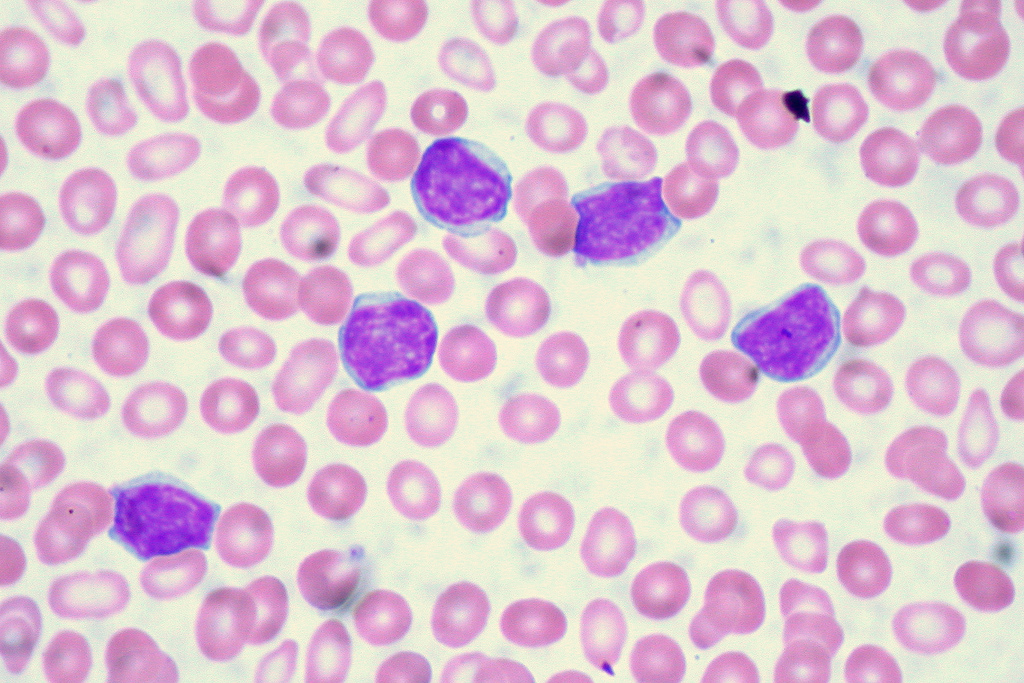
\includegraphics[width=1\linewidth,height=200px,]{./images/2-blood-smear} 

}

\caption{Microscopic image of blood smear containing lymphocytes (purple, with granulated nuclei) (Source: Euthman, https://www.flickr.com/photos/euthman/2869815349 )}\label{Fig. unnamed-chunk-1}
\end{figure}

As blood smear image examination is a tedious and time consuming process
(Naugler et al. 2014), many algorithms have been developed to automate
the process. Image recognition and segmentation is used to prepare the
input, sually dividing the cell image into masks. A cell mask is
produced, by selecting the cell in between all of the complex elements
of the image. The cell is then divided into semantically significant
regions (\emph{e.g.} nucleus mask or cytoplasm mask) through image
segmentation, via techniques like the \emph{Watershed Algorithm} or
machine learning algorithms like \emph{Support Vector Machines (SVMs)}.
This image processing step is crucial for a good classification
workflow, as it prepares the input for the following steps.

The next step is feature selection/extraction, in which a group of
features is measured in order to use these quantitative values for
classification. Good features must be informative. Features that largely
overlap between classes don't offer a significant amount of
distinctiveness, Becuase of this, the features selected or extracted
must be \textbf{very similar inside the same class} and
\textbf{distinctive between classes}. White blood cells are wildly
different between them, varying substantially between cell families, and
even if there are features that are observably different between
families, \textbf{not all features} will be significant for a
classification task.

The last step is the classification itself. Classification demands for a
pattern to be established that can reliably assign a given sample to a
given class. There are many machine learning algorithms used to find
these patterns, such as \emph{ANN's} or \emph{SVMs}. For the purposes of
this project, a focus will be given to \emph{SVMs}.

\emph{Support Vector Machines} are a machine learning algorithm first
introduced by Vladimir Vapnik (Leslie, Eskin, and Noble 2002). They aim
to find one or a set of hyperplanes that divide the sample space into
categories, as cleanly as possible and with as little interference of
samples from one space into another. This or these hyperplanes are then
used to classify new test samples into one of the original classe.

In a non-ideal, more realistic background, samples won't be always
cleanly separated into smooth groups. This situation is managed by
searching for a compromise between maximum classification accuracy and a
reasonable classification error. Different \emph{kernels} can also be
introduced in the \emph{SVM} algorithm in order to improve the
classification results.

The morphological features of peripheral blood cells were first
translated into a mathematical scoring system by Benattar and Flandrin
(Benattar and Flandrin 2001). Mathematical measurement of these features
induces intraobserver and interobserver objectivity and allows for a
quantitative assesment of cell features, being the ones in abnormal
lymphocytes the most difficult to identify. Thus, mathematical
morphology tools have been developed with the aim of processing
peripheral blood images and extracting and processing sets of features
which are then used to classify the cell. These features need to be
constructed and optimized for best performance and accuracy of the
derived classification, or, in some cases, risk being affected by the
\emph{Curse of Dimensionality}.

The \emph{Curse of Dimensionality} is a common problem for many data
analysis fields, in that as the dimensionality (number of observed
features, or number of dimensions) of the data grows, the analytic space
grows exponentially with each added dimension; even though the initial
number of samples may be optimized for a study, the real quantity of
information quickly grows ``sparse'' as the dimensionality of the study
grows. In many \emph{nearest neighbor} approaches to data analysis this
problem is buffered by the fact that \emph{significant} new dimensions
also offer more contrast between points, so it is those \emph{noise}
dimensions that need to be identified and suppressed.

This can be managed by dimension reduction methods, as it has been in
(Puigv{í} et al. 2017) and (Alf{é}rez 2015). The most complete set of
features is described in detail in the former, in the \emph{Materials
and Methods} section. In this study, a total of 325 patients were
included (Fig.2), for a total of 12574 cell images. This images were
obtained using the CellaVision DM96.

\begin{figure}[h]

{\centering 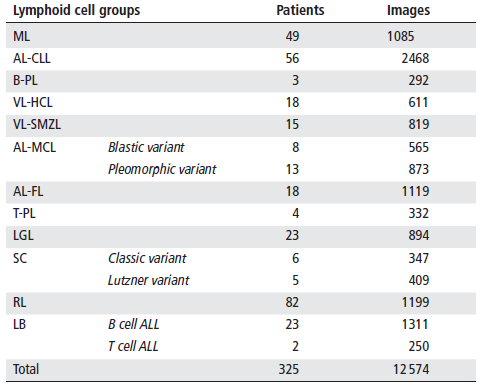
\includegraphics[height=200px,]{./images/4-distribution-images} 

}

\caption{Distribution of lymphoid cell groups, number of patients and images included in the study (Source: Puigví et al.)}\label{Fig. distribution}
\end{figure}

Three \emph{ROIs} (Regions of Interest) are obtained (nucleus, whole
cell and peripheral zone around the cell), and a fourth \emph{ROI} is
obtained as the difference between cell and nucleus regions (Fig.3).
Features are divided in geometric features and color-texture features,
all of them measured quantitatively.

\begin{figure}[h]

{\centering 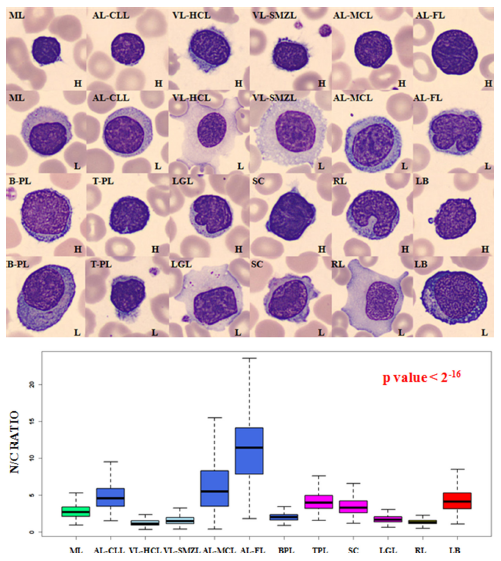
\includegraphics[width=6in,height=200px,]{./images/3-nc-ratio} 

}

\caption{Examples of different cells, showing differential nucleus/cytoplasm ratio, with associated boxplots (Source: Puigví et al.)}\label{Fig. ncratio}
\end{figure}

All in all, 27 geometric features (including \textbf{area},
\textbf{perimeter} and \textbf{N/C ratio}) and 2649 colour-texture
features (43 texture features applied through six colour spaces:
\textbf{RGB}, \textbf{CMYK}, \textbf{XYZ}, \textbf{Lab}, \textbf{Luv}
and \textbf{HSV}) are extracted, for a total of 2676 features.

\begin{figure}[h]

{\centering 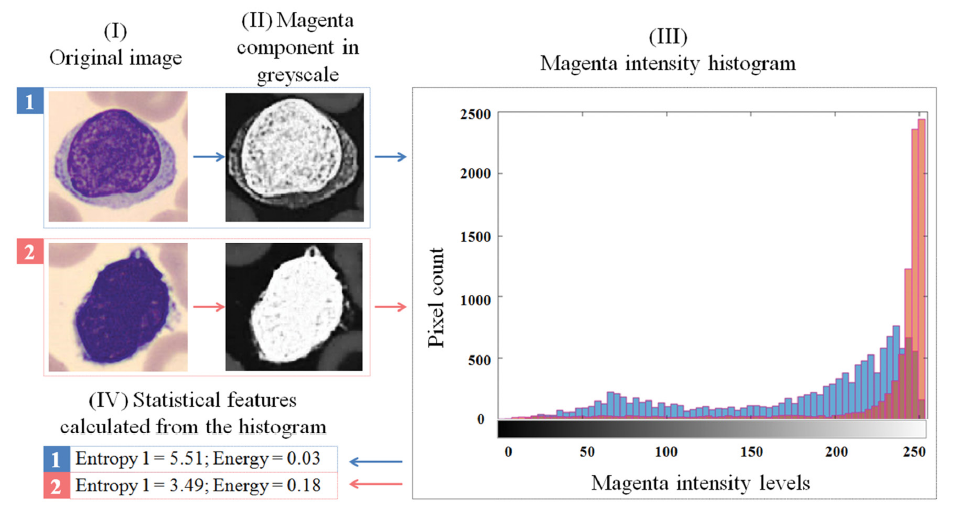
\includegraphics[width=1\linewidth,height=200px,]{./images/1-grayscale-intensity-lymph} 

}

\caption{Magenta component grayscale decomposition and associated histogram (Source: Puigví et al.)}\label{Fig. grayscale}
\end{figure}

The problem of dimensionality is solved through dimension reduction
techniques (theoretic feature selection), decreasing the number of
features to a more relevant, less redundant subset of 20 features
(Fig.5), and malignant diagnoses were confirmed following the WHO
classification.

\begin{figure}[h]

{\centering 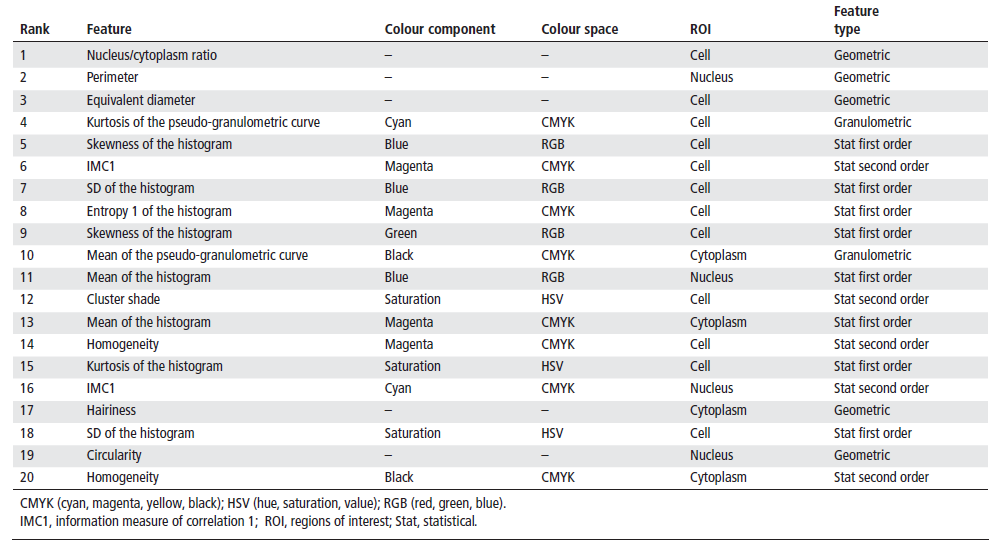
\includegraphics[width=6in,height=200px,]{./images/5-relevant-features} 

}

\caption{20 most relevant, less redundant features selected (Source: Puigví et al.)}\label{Fig. relevant_features}
\end{figure}

Data analysis was performed with \textbf{R} code, validating for
residual normality through Kolmogorov-Smirnov, homocedasticity through
Flingner-Killeen, significance through Kruskal-Wallis and multiple
comparisons through Kruskal-Wallis after Dunn tests applying a Bonferoni
adjustment.

The selected features allowed for the quantification of different
morphological characteristics with significant p-values, being \emph{N/C
ratio} the best feature for distinction.

As has been mentioned, the correct diagnosis of lymphoma offers a
significant survival rate, an as such, every single step of the
classification protocol should be optimised for best performance, both
in terms of accuracy and costs. Thus, the justification for this project
on a scientific level is to compare the feasibility of several dimension
reduction techniques applied to the classification of lymphoma. This
comparison will be made through an accuracy scoring result.

The accuracy of a prediction is the proportion of true positives plus
true negatives against the total prediction result. It measures the
amount of cases in which the observed results matched the expected
results. Errors in prediction may or may not have the same ``weight''
for a given problem (as an example, a false positive in cancer diagnosis
may raise an unnecesary alarm; a false negative may cause a lack of
treatment and so, a serious health issue). This project will, through
understanding of the context of the mentioned study, establish an
accuracy scoring system, determine if different errors have different
costs, compare scores, and analyse the results for conclussions both on
comparison of techniques and the implications of the scoring system.

\subsection{1.2 - Project goals}\label{project-goals}

\subsubsection{1.2.1 - General goals}\label{general-goals}

The goal of this project is to \textbf{compare several techniques of
dimension reduction} through the construction of significant features
and their respective results given a classification workflow. This
classification workflow should differentiate normal, abnormal and
reactive lymphoid cells. The resulting accuracy values will serve as
scoring for the features constructed, and as such, for the objective
assesment of the behaviour of the dimension reduction techniques behind
them.

\subsubsection{1.2.2 - Specific goals}\label{specific-goals}

\textbf{Specific goals for Phase 1 (17-10-2017 through 20-11-2017)}

1 - To design a \textbf{comparison protocol} for different dimension
reduction techniques.

1.1 - To research, understand, brief on, and choose an array of
dimension reduction techniques for comparison.

1.2 - To choose a programming environment to work with (languages,
frameworks\ldots{})

1.3 - To assess the methods of, understand and ultimately extract a
subset of functions from the appointed languages and frameworks to apply
to the test data.

\textbf{Specific goals for Phase 2 (21-11-2017 through 18-12-2017)}

2 - To apply this protocol to each technique within the frame of
lymphocyte classification, achieving an \textbf{objectively quantifiable
scoring system}.

2.1 - To set a scoring system to satisfy the need for an objective
measure of accuracy. This scoring system will include weighing of types
of errors.

2.2 - To apply each of the selected dimension reduction techniques,
under equivalent parameters, to the test data.

2.3 - To classify the behaviour of the referred techniques, based on the
selected scoring system, as applied to the stated problem (lymphocyte
classification)

\subsection{1.3 - Focus and followed
method}\label{focus-and-followed-method}

Given the specific goal of this project (the comparison of dimension
reduction techniques), the focus to accomplish it will be directed to
the evaluation of the accuracy of classification tasks implementing each
of these techniques. Feature construction aims to explain the most
variance through the less possible, most explicative, features. For a
constant given amount of variance explained through variables in a
classification task, the accuracy of the predicted classes improves
while the number of dimensions decreases.

The methods to accomplish this will be a selection of dimension
reduction techniques, including \textbf{PCA}, \textbf{ICA} and
\textbf{Factor Analysis} amongst others, applied to the problem dataset
and used as input for the same machine learning classification algorithm
(SVM with an RBG kernel).

This method has been evaluated as the most appropriate, as it makes it
possible to subject the objects of evaluation to an equal environment,
under equal conditions, and give out a numerical, objective measure of
correlation with observed results.

\subsection{1.4 - Project plan}\label{project-plan}

\subsubsection{1.4.1 - Tasks}\label{tasks}

\textbf{Tasks for Phase 1:}

1.1.1 - Choose a subset from the most used and widely applied dimension
reduction techniques appliable to the present topic, including
\textbf{PCA}, \textbf{ICA} and \textbf{Factor Analysis}. (1 week, 21
hours equivalent)

1.2.1 - Elaborate a list of widely bioinformatics-applied languages (and
frameworks, if used within one). (7 days, 21 hours equivalent)

1.2.2 - Choose a subset from those languages and frameworks and
elaborate a briefing of characteristics and examples of application. (3
days, 9 hours equivalent)

1.3.1 - Elaborate a list of dimension reduction packages and functions
from chosen languages. (7 days, 21 hours equivalent)

1.3.2 - Choose a subset and elaborate a briefing of package traits:
optimal application, parameters, example workflows it has actually been
used for, etc. (4 days, 12 hours equivalent)

1.3.3 - Elaborate monitoring report for \textbf{Phase 1}. (7 days, 21
hours equivalent)

\textbf{Tasks for Phase 2:}

2.1.1 - Elaborate a short briefing on the value of prediction accuracy
as output by this packages. (4 days, 12 hours equivalent)

2.1.2 - Assess the validity of it for all the packages selected, and, if
it is not valid for all of them, extrapolate a valid, normalized scoring
system. (6 days, 18 hours equivalent)

2.2.1 - Apply each and every package's or function's workflow to the
supplied lymphocyte data. (4 days, 12 hours equivalent)

2.3.1 - Present the score output of each of the applications in a
user-friendly manner. (3 days, 9 hours equivalent)

2.3.2 - Extract behaviour/comparison conclussions from this score
output. (4 days, 12 hours equivalent)

2.3.3 - Elaborate monitoring report for \textbf{Phase 2}. (8 days, 24
hours equivalent)

\subsubsection{1.4.2 - Calendar}\label{calendar}

The following Gantt diagram represents the division of time through the
proccess of this project:

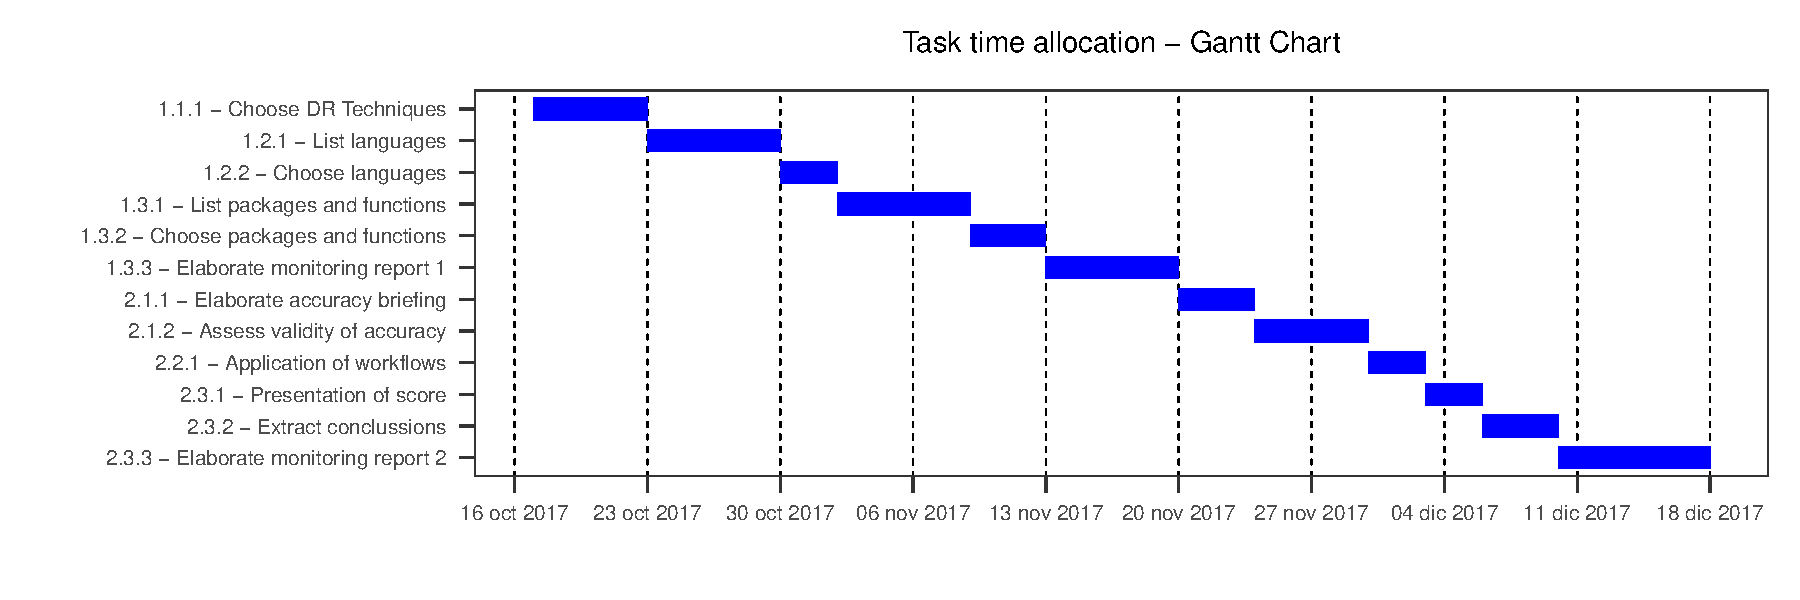
\includegraphics[height=200px,]{gimenezGredillaDaniel-TFM-REPORT_files/figure-latex/calendar-1}

\subsubsection{1.4.3 - Milestones}\label{milestones}

The following tables represent the milestones for each development
phase.

\begin{longtable}[c]{@{}ll@{}}
\caption{Phase 1 milestones}\tabularnewline
\toprule
Deadline & Milestone\tabularnewline
\midrule
\endfirsthead
\toprule
Deadline & Milestone\tabularnewline
\midrule
\endhead
01-NOV-2017 & Array of candidate bioinformatics languages, tools and
protocols assessed\tabularnewline
20-NOV-2017 & Definitive subset of bioinformatics languages, tools and
protocols selected\tabularnewline
20-NOV-2017 & Monitoring report for Phase 1\tabularnewline
\bottomrule
\end{longtable}

\begin{longtable}[c]{@{}ll@{}}
\caption{Phase 2 milestones}\tabularnewline
\toprule
Deadline & Milestone\tabularnewline
\midrule
\endfirsthead
\toprule
Deadline & Milestone\tabularnewline
\midrule
\endhead
28-NOV-2017 & Scoring system completely defined\tabularnewline
08-DEC-2017 & Complete set of workflows applied\tabularnewline
18-DEC-2017 & Behaviour/comparison conclussions from output
elaborated\tabularnewline
18-DEC-2017 & Monitoring report for Phase 2\tabularnewline
\bottomrule
\end{longtable}

\begin{longtable}[c]{@{}ll@{}}
\caption{Post-production milestones}\tabularnewline
\toprule
Deadline & Milestone\tabularnewline
\midrule
\endfirsthead
\toprule
Deadline & Milestone\tabularnewline
\midrule
\endhead
02-JAN-2018 & Final report produced and delivered\tabularnewline
10-JAN-2018 & Virtual presentation produced and delivered\tabularnewline
\bottomrule
\end{longtable}

\subsubsection{1.4.4 - Risk analysis}\label{risk-analysis}

Some of the factors that could hinder the proposed work frames are the
following:

\begin{enumerate}
\def\labelenumi{\arabic{enumi}.}
\item
  Technical problems: a short buffer of time must be allocated for
  unexpected technical problems stemming from equipment malfunction,
  infrastructure breakdown, etc. Measures covering these problems
  include a recurrent backup system, cloud storage and accessibility to
  the project and its resources from several, if controlled,
  workstations.
\item
  Goal overextension: an incorrect or exaggerated choice of dimension
  reduction techniques or an overambitious reach could mean an
  ineffective use of time. This is controlled by allocating an initial
  time for a detailed judgement and selection of techniques to include
  in this project's comparison goal.
\item
  Incompatibilities: accuracy measurements between packages or functions
  in different languages or frameworks could demonstrate to be
  incompatible between them, or not fit to compare; this is avoided
  through both the allocation of time for a strict selection of these
  languages and frameworks, and for the production of a normalized
  scoring system.
\end{enumerate}

Although there are many other factors that could mean an obstacle for
the correct development of each phase, they are not foreseeable and,
thus, to be assessed on an occurrence basis.

\subsubsection{1.4.5 - Associated project
costs}\label{associated-project-costs}

Economical costs for the present project will be only those associated
with infrastructural uses (power and time used for computation), as all
implemented software will be Open Source.

\subsubsection{1.4.6 - Ethical and legal data
implications}\label{ethical-and-legal-data-implications}

All data included in this project is anonymous and carries no risk for
specific study patients. Even so, no data set will be made available for
the public, and all computation and data presented will be in the form
of final results in which no specific person will be addressed.

\subsubsection{1.4.7 - Briefing: first monitoring report - November
2017}\label{briefing-first-monitoring-report---november-2017}

\textbf{Development state:}

Up to this date, a complete background for the project has been
researched. The goal of the project is clear, and a good wealth of
literature on the topic and multiple sub-topics at hand has been sought,
found and studied. The ups and downs of both dimension reduction
techniques and programming languages and packages have been assessed,
evaluated and discriminated. The redaction of a complete report is on
its way, and the general state of development is in accordance with both
the official timetables and the personally scheduled tasks.

\textbf{Undertaken tasks:}

1.1.1 - Choose a subset from the most used and widely applied dimension
reduction techniques appliable to the present topic, including
\textbf{PCA}, \textbf{ICA} and \textbf{Factor Analysis}. (1 week, 21
hours equivalent)

\textbf{State: Complete - In schedule.} Two additional techniques
(\textbf{Autoencoders} and \textbf{T-distributed Stochastic Neighbor
Embedding}) have been added to the pool for the reasons stated in the
report.

1.2.1 - Elaborate a list of widely bioinformatics-applied languages (and
frameworks, if used within one). (7 days, 21 hours equivalent)

\textbf{State: Complete - In schedule.} Languages such as \textbf{SPSS},
\textbf{Matlab} or \textbf{Haskell} have been assessed and evaluated for
their usefulness and fit to the goals of this project.

1.2.2 - Choose a subset from those languages and frameworks and
elaborate a briefing of characteristics and examples of application. (3
days, 9 hours equivalent)

\textbf{State: Complete - In schedule.} The final candidates for
comparison, due to the factors described in the project, are Python and
R.

1.3.1 - Elaborate a list of dimension reduction packages and functions
from chosen languages. (7 days, 21 hours equivalent)

\textbf{State: Complete - In schedule.}

1.3.2 - Choose a subset and elaborate a briefing of package traits:
optimal application, parameters, example workflows it has actually been
used for, etc. (4 days, 12 hours equivalent)

\textbf{State: Complete - In schedule.} The chosen packages have been
listed with a historical and mathematical background where appliable,
and reasons for selection.

1.3.3 - Elaborate monitoring report for \textbf{Phase 1}. (7 days, 21
hours equivalent)

\textbf{State: Complete - In schedule.}

\textbf{Incomplete tasks:}

As of this monitoring report there are no incomplete tasks.

\textbf{Hindrances and unforeseen circumstances:}

There have been neither hindrances nor unforeseen circumstances.

\textbf{Update - milestones:}

Up to this date, the original milestones still apply, as stated in the
following table:

\begin{longtable}[c]{@{}ll@{}}
\caption{Phase 1 milestones}\tabularnewline
\toprule
Deadline & Milestone\tabularnewline
\midrule
\endfirsthead
\toprule
Deadline & Milestone\tabularnewline
\midrule
\endhead
01-NOV-2017 & Array of candidate bioinformatics languages, tools and
protocols assessed\tabularnewline
20-NOV-2017 & Definitive subset of bioinformatics languages, tools and
protocols selected\tabularnewline
20-NOV-2017 & Monitoring report for Phase 1\tabularnewline
\bottomrule
\end{longtable}

All milestones have been completed and the grounds for the second phase
of the project are established.

\textbf{List of products:}

Given the development state of the project, in which a theoretical
background has been stated and tools have been selected, the only
product for this phase is the current monitoring report. It is expected,
as part of the project's plan, that the second phase will yield the
final products.

\subsubsection{1.4.8 - Briefing: second monitoring report - December
2017}\label{briefing-second-monitoring-report---december-2017}

\textbf{Development state:}

The project's tasks have been largely completed by this point, given
some extra tasks that are detailed here and unforeseen circumstances and
hindrances that were buffered through corrective or paliative action.

\textbf{Undertaken tasks:}

2.1.1 - Elaborate a short briefing on the value of prediction accuracy
as output by this packages. (4 days, 12 hours equivalent)

\textbf{State: Complete - In schedule.}

2.1.2 - Assess the validity of it for all the packages selected, and, if
it is not valid for all of them, extrapolate a valid, normalized scoring
system. (6 days, 18 hours equivalent)

\textbf{State: Complete - In schedule.}

2.2.1 - Apply each and every package's or function's workflow to the
supplied lymphocyte data. (4 days, 12 hours equivalent)

\textbf{State: Complete - Out of schedule.}

2.3.1 - Present the score output of each of the applications in a
user-friendly manner. (3 days, 9 hours equivalent)

\textbf{State: Complete - Out of schedule.}

2.3.2 - Extract behaviour/comparison conclussions from this score
output. (4 days, 12 hours equivalent)

\textbf{State: Complete - Out of schedule.}

2.3.3 - Elaborate monitoring report for \textbf{Phase 2}. (8 days, 24
hours equivalent)

\textbf{State: Complete - Out of schedule.}

\textbf{Unscheduled activities}

As part of the tasks undertaken, it has been necessary to upgrade the
technical resources available to the author. The machine in which the
project's computation is run is a \textbf{Hewlett Packard Proliant Gen
8} microserver. It has proven reliable and sturdy, but not powerful
enough for some of the proceedings. As such, more RAM and a more
powerful processor were acquired and the server was modded with them.
This process took the best part of two days of work, from November 30th
through December 2nd.

\textbf{Incomplete tasks:}

There were no incomplete tasks.

\textbf{Hindrances and unforeseen circumstances:}

In the original planning, possible sources of deviation and obstacles
were proposed as:

\textbf{1. Technical problems:} A single, important technical problem
has arised when undertaking the second phase of this project: computing
power. For some of the dimensional reduction techniques (\textbf{PCA}
and \textbf{ICA}) the processing times and virtual memory requirements
were met even under the most stringent parameters. On the other hand,
some of the least tried or most resource-heavy techniques
(\textbf{Stacked Denoising Autoencoders} and \textbf{T-Stochastic
Neighbor Embedding}) repeatedly hit a technical roof which hindered the
progress of this project.

\textbf{2. Goal overextension:} no problems associated with
overextension have arised. The scheduled objectives have been deemed by
the author as realistic and, apart from other hindrances, achievable.

\textbf{3. Incompatibilities:} no incompatibilities have been found
neither in practice nor in literature.

As such, technical buffering measures were undertaken. In the first
place, method optimisation techniques were tested, such as the use of
resource-light variable structures as turning data frames into sparse
matrices or garbage-collection methods after each iteration of the
processes, but none of them lowered the requirements in a manner
significant enough to be able to complete them to satisfaction.

As this was clearly a hard-cap problem, an \textbf{Intel® Xeon®
E3-1265L} processor, and two 8Gb \textbf{Kingston DIMM 1600 Mhz 240
pins} RAM chips were acquired in order to be able to parallelize
processing and provide the machine with a higher virtual memory roof.
This microserver modification took the best part of two days of work and
brought with it a total blackout in computing during this time. This
blackout time was put to use in redaction and problem-solving research.

\textbf{Update - milestones:}

With the briefed hindrances in mind, the original milestone table is
updated as follows:

\begin{longtable}[c]{@{}ll@{}}
\caption{Phase 2 milestones}\tabularnewline
\toprule
Deadline & Milestone\tabularnewline
\midrule
\endfirsthead
\toprule
Deadline & Milestone\tabularnewline
\midrule
\endhead
28-NOV-2017 & Scoring system completely defined\tabularnewline
08-DEC-2017 & Complete set of workflows applied\tabularnewline
18-DEC-2017 & Behaviour/comparison conclussions from output
elaborated\tabularnewline
18-DEC-2017 & Monitoring report for Phase 2\tabularnewline
\bottomrule
\end{longtable}

\subsubsection{1.4.9 - Final Gantt Diagram (after
alterations)}\label{final-gantt-diagram-after-alterations}

Referring to the original the Gantt diagram presented within the initial
plan:

\includegraphics[height=200px,]{gimenezGredillaDaniel-TFM-REPORT_files/figure-latex/calendar_2-1}

The planned tasks were slowed down by the aforementioned technical
problem. Deviations were mainly focused in \textbf{task 2.2.1 -
Application of workflows}. The unplanned use of two days was distributed
evenly amongst all the following tasks, so the original Gantt diagram is
recast as follows:

\includegraphics[height=200px,]{gimenezGredillaDaniel-TFM-REPORT_files/figure-latex/new_calendar-1}

\subsection{1.5 - Brief summary of products
obtained}\label{brief-summary-of-products-obtained}

\subsubsection{1.5.1 - Work plan}\label{work-plan}

A document pertaining the project's planification will be delivered by
October the \(16^{th}\), this being it. This document's aim is to
reflect the project's expected goals and tasks to accomplish and the
time frames in which to fit them. Pragmatism is expected in this
planning, meaning the ability to fit realistic goals and tasks in
realistic timeframes, acknowledge possible hindrances and obstacles, and
establishing procedures to avoid or sort them out.

This project's work plan is been rendered via R, using packages
\textbf{Rmarkdown}, \textbf{ggplot2}, \textbf{knitr}, and
\textbf{reshape2}. The embedded Gantt graph is produced via
\textbf{ggplot2} and \textbf{reshape2}, from an input of tasks in data
frame format and a series of graphic parameters.

This document will also establish the products that will stem from the
project, any additional outputs, and the monitoring and evaluation
thereof.

\subsubsection{1.5.2 - Report}\label{report}

Three reports will be made through this project's duration, structured
as follows:

The first document will be a monitoring report, due November the
\(20^{th}\), in which the project's ongoing evolution will be described.
This will be composed of the description itself, a complete relation of
overtaken activities, both foreseen and unforeseen, a relation of
hindrances and obstacles and the measures taken to buffer them, complete
with an update of time frames, a list of delivered partial results and
any particular comment by the project's tutor.

Another monitoring report, due December the \(18^{th}\), will be
generated with contents similar to the first one, this time with a focus
on the completed second phase of the project and the degree of
accomplishment of the planned goals for it.

The final report, due January the \(2^{nd}\), with a maximum length of
90 pages, will present the output of the project, with a justification
of its interest, goals, methodology and materials, and results obtained.

\subsubsection{1.5.3 - Product}\label{product}

In the course of this project, an automated comparison report script
will be produced. The code used will be added as an addendum to the
final report, along with code comments and protocols of use. The code
will be stored in a GitHub repository, available for the public to
clone, review and use. GitHub is a version-control platform used to
store git repositories, with an emphasis on open-source, collaborative
efforts and project versioning. Mendeley will be used as referencing
tool, syncronized with R Markup through an embedded \emph{.bib} file.

\subsubsection{1.5.4 - Virtual presentation}\label{virtual-presentation}

The virtual presentation for this project will be carried out through
Present@, a presentation tool offered by \textbf{Universitat Oberta de
Catalunya} for the display of project results. This presentation will be
comprised of approximately 20 slides with an oral presentation for a
maximum of 20 minutes. This presentation's aim is to be as concise and
informational as possible, while delivering the results and conclussions
of the project in a clean, outreaching way.\\The presentation will be
produced between the \(3^{rd}\) and \(10^{th}\) of January 2018, January
the \(10^{th}\) being the deadline. Of special importance is the
content, synthetic ability and clarity of purpose and expression.
Evaluation criteria have been provided by the project's tutor.

\subsubsection{1.5.5 - Project
self-evaluation}\label{project-self-evaluation}

This project's self-evaluation will confront it from two angles: first,
a side-by-side comparison of initial goals and time schedules and final,
actual results and time schedules, and second, a thorough analysis of
style, clarity and informative value. Being this:

\textbf{Goals and schedules:}\\1 - Correct assertion of techniques to
compare: the techniques assessed are widely used, available to the
general research personnel, and suited for the task at hand. Also, the
number of techniques is decided pragmatically, avoiding overextension
and, thus, decrease in effective time. 2 - Validity of scoring system
and conclussions: the scoring system is, by itself or through
normalisation, fit to give an objective, comparable value. The
conclussions that follow are in agreement with this scoring system. 3 -
Adecuation of assigned times: the assigned times corresponded to the
times actually employed for each task, and so, milestones are
accomplished within the expected period.

\textbf{Style and structure:}\\1 - Style: the project is easily
readable, is expressed in a correct way, follows correct style
guidelines, quotes and references are strictly marked.\\2 - Structure:
the project follows the structure established by the documentation
provided through the subject. Contents are correctly divided in
sections. The project as a whole presents a semantic flow without
logical leaps that may hinder the reader's comprehension.

\subsection{1.6 - Brief description of other
chapters}\label{brief-description-of-other-chapters}

\textbf{2 - Dimension reduction: an introduction}: A brief presentation
of the main topic for this project. What they are, what they are useful
for.

\textbf{2.1 - PCA}: Historical and mathematical background of this
technique, and reasons for its selection.

\textbf{2.2 - ICA}: Historical and mathematical background of this
technique, and reasons for its selection.

\textbf{2.3 - Factor Analysis}: Historical and mathematical background
of this technique, and reasons for its selection.

\textbf{2.3 - Autoencoders}: Historical and mathematical background of
this technique, and reasons for its selection.

\textbf{2.4 - T-distributed Stochastic Neighbor Embedding}: Mathematical
background of this technique, and reasons for its selection.

\textbf{2.5 - LDA}: Historical and mathematical background of this
technique, and reasons for its selection.

\textbf{3 - Tools}: Languages and packages used for this project.

\textbf{3.1 - Criteria}: Criteria through which these tools were
selected.

\textbf{3.2 - Python}: History, modules and implementations from this
language used for the current project.

\textbf{3.3 - R}: History, packages and libraries and implementations
from this language used for the current project.

\textbf{4 - Comparative Scoring}: Assessment of an objective, measurable
way to compare dimension reduction techniques.

\textbf{4.1 - Classification Accuracy Metrics}: A general look at the
ways in which prediction accuracy is measured.

\textbf{4.2 - Binary Classification Versus Multiclass Classification
Metrics}: On how different accuracy metrics are best suited to
evaluating classifiers with two classes or more.

\textbf{4.3 - Classification Rate}: Focus on this multiclass accuracy
metric.

\textbf{4.4 - Cohen's Kappa}: In-depth look at this multiclass accuracy
metric.

\textbf{4.5 - Chosen Scoring Metric}: The metric to be used in this
project and reasons for it.

\textbf{5 - Comparison Methods and Protocols}: Previously explained
techniques and implementations, put to work.

\textbf{5.1 - Introduction and General Data Set Description}: A brief
introduction to the data being treated, and ways to sort out imbalance.

\textbf{5.2 - Goals and techniques}: Brief resume of techniques being
implemented.

\textbf{5.3 - Dimension Reduction techniques - R}: \textbf{R}
implementations of the selected dimension reduction techniques.

\textbf{5.4 - Dimension Reduction techniques - Python}: \textbf{Python}
implementations of the selected dimension reduction techniques.

\section{2 - Dimension reduction: an
introduction}\label{dimension-reduction-an-introduction}

Actual data derived from actual studies, as opposed to ideal,
condition-controled data, is mudded by the complexity of reality, and in
order to approximate it, needs to be measured by large quantities of
variables, giving up high dimensionality datasets, as may be the case of
digital imaging, speech recognition or complex classification tasks.
This high dimensionality needs to be adequately reduced in order to make
studies attainable, able to be handled effectively. In fact, not all the
measured variables may be ``important'' to the goal of a study.

This can be mathematically formulated as follows (Fodor 2002):

Given the \emph{p}-dimensional random variable
\(x = (x_1,...,x_p)^{T}\), we need to find a lower dimensional
representation of it, \(s = (s_1,...,s_k)^T\) with \(k \le p\) that
captures the information in the original data.

Ideally, this involves constructing a representation of the data
according to its intrinsic dimensionality. The intrinsic dimensionality
of data is the minimum number of parameters needed to account for the
oberserved properties of the data ({Van Der Maaten}, Postma, and {Van
Den Herik} 2009). As a result, many techniques have been developed, both
supervised and unsupervised, to handle the construction of this
representation.

Traditionally, dimensionality reduction techniques relied in linear
transformations, like those used in \emph{PCA} (Principal Component
Analysis), Factor Analysis or classical scaling. Linear techniques
result in newly constructed features that are a linear combination of
the originals. However, given that in many fields, complex, nonlinear
data is obtained, many other nonlinear methods have been developed, like
Autoencoders, nonlinear applications of \emph{PCA}, Kernel \emph{PCA},
Laplacian Eigenmaps, etc.

The techniques used for this project will be described in the next
subsections. History, mathematical background and reasons for its
selection will be addressed where available. Further along this
document, programming applications and protocols will be addressed.

\subsection{2.1 - PCA}\label{pca}

PCA is the most used unsupervised, linear dimension reduction technique
currently available. It is also the best, in the mean-square error sense
(Fodor 2002). Its central idea is the construction of a set of features
from a number of initial variables (Jolliffe 2002). The number of new
features will be less than the initial variables, while retaining as
much as possible of the initial variation. This is achieved by linear
transformations of the original data, and then establishing a descending
order of the new features attending to the amount of variation retained
or explained by each of them.

Given \(X\), a vector of \emph{p} random variables, as object of
interest for any study, and given that \(X\) is complex enough, the raw
study of the correlation between variables may get to be inefficient and
expensive in time and effort. Instead of getting the \emph{p} variances
and the \(\frac{1}{2}p(p -1)\) correlations for each sample in the
study, the goal is to search for less, equally (or effectively equally)
explicative features.

\subsubsection{2.1.1 - Historical
background}\label{historical-background}

PCA was invented in 1901 by Karl Pearson, the roots of it deeply
burrowed in regression-thinking. In its first approach, which
independently builds up on singular value decomposition, Pearson is
concerned with finding lines and planes that best fit a set of points in
a \(p\)-dimensional space through geometric optimization (Jolliffe
2002).

It has been mathematically reinterpreted several times along its
history. In the thirties, Hotelling takes his own approach. He
introduces the term ``components'', as ``factors'', which is used in
psychological literature, may create confussion with other mathematical
uses of this word. His motivation is the thought that there may be a
smaller set of derived variables that explain the values of the original
variables. It is his own interpretation that coins the term ``method of
principal components''.

Hotelling gives more weight to the Principal Components axis'
directions, in a much more multivariate statistical approach. In
Hotelling's approach he defines the Principal Axis Property: the first
component explains the most variation, the second component the second
most variation, and so on. The first Principal Components define new
axis to be taken into account for the next Principal Components. This
means a rotation of the subspace has an effect on the resulting
Principal Components (Bro and Smilde 2014).

From then on further applications and extensions of PCA have been made
by researchers such as \textbf{Anderson} (1963), \textbf{Gower} (1966)
or \textbf{Jeffers} (1967).

Even though it seems to be a simple technique and much has been
discussed about it, it has been applied to an extensive range of fields
and is still in research.

\subsubsection{2.1.2 - Mathematical
background}\label{mathematical-background}

Let us suppose data is collected in a matrix \(X\) with \(I\) rows
\((i = 1,...,I)\). These \(I\) rows will usually be the observations or
samples for the study. \(X\) is also composed of \(J\) columns
\((j = 1,...,J)\), being these the measured variables. Each of these
variables are denoted \(x_j (j=1,...,J)\), and thus the matrix is of
\(I x J\) dimensions.

The linear combination of these variables can be written as
\(t = w_1 * x_1 + ... + w_J * x_J\). The new vector \(t\) is in the same
\emph{I}-dimensional space as the original variables, and it is a linear
transformation of these variables. This can be expressed, in matrix
notation, as \(t = wX\), \(w\) being the linear factor vector with
elements \(w_j (j = 1,..., J)\) (Bro and Smilde 2014).

As has been explained in former sections, as much information of \(X\)
should be carried on to \(t\) as possible. With enough of that
information preserved, \(t\) acts as a good summary of \(X\). This
information can be expressed as variance, \(var(t)\).

Variance, \(s^2\), is statistically almost identical to standard
deviation (SD) (Smith 2002). The formula for variance is:

\(s^2 = \frac{\sum_{i=1}^n(X_i - \bar{X})^2}{n - 1}\)

Being this just the squared SD.

So the goal is to choose a linear transformer \(w_1,...,w_J\) such that
this \(var(t)\) is maximized. Given that measures are subject to number
sizes according to their own background, they need to be scaled down to
a comparable scale, such that \(w\) may really be appliable with
significant results unaffected by arbitrary size changes.

So, the problem can be expressed as
\(\underset{||w|| = 1}{\operatorname{argmax}} var(t)\).

\(argmax\) being the argument \(w\) of length 1 that maximizes
\(var(t)\). Returning to matrix notation, and going back to the equation
\(t = wX\), the can be equaled to:

\(\underset{||w|| = 1}{\operatorname{argmax}} (t^Tt) = \underset{||w|| = 1}{\operatorname{argmax}} (w^TX^TXw)\)

Which can be solved as an eigenvector problem, being the first
eigenvector the first Principal Component, the second eigenvector the
second Principal Component, and so on.

\subsubsection{2.1.3 - Reasons for
selection}\label{reasons-for-selection}

PCA is an ubiquitous technique that is described and analyzed, in any of
its many interpretations, almost in every book about feature analysis
(Tipping and Bishop 1999). It's a widely used linear dimension reduction
technique that has proven itself of the utmost power time and time
again. As such, including it in this comparison is useful not only for
the comparison of the technique itself, but as a kind of benchmark: to
asses any dimension reduction technique that, applied to the subject of
this study (feature construction for lymphocyte classification), is able
to hold a candle to PCA.

Also, as has been stated, PCA has been focused on from many angles, and
it is expected to have been widely tackled by bioinformatics languages
and tools. A suitable bioinformatics integration of this technique is
expected to be found, or several, that fit this study for comparison; in
an ideal context, it should be accessible, Open Source and the methods
and results of this study should be easily reproducible by anyone
reviewing it.

\subsection{2.2 - ICA}\label{ica}

Independent Component Analysis (\emph{ICA}) is a statistical method for
transforming an observed multidimensional random vector into components
that are statisticaly as independent from each other as possible, this
is, a tendency to \textbf{redundancy reduction} (Tobergte and Curtis
2013). In its linear approach, as with other dimension reduction
algorithms, its goal is to take a zero-mean, \emph{m}-dimensional
variable, and by means of a linear transformation, find its
\emph{n}-dimensional transform, such that \(n \le m\), this
transformation having some suitable properties. The vectors obtained
from this transformation are neither orthogonal nor ranked in order.

Feature extraction is a prominent application of \emph{ICA}. It is
originally motivated by results in neuroscience that suggest that the
same cited principle of redundancy reduction is applied by the brain for
the early processing of sensory data.

\emph{ICA} is a generative model (it describes how the observed data are
generated by describing the components), and it seeks the minimization
of mutual information between the transformed variables. It depends on
the supposition of nongaussianity for the data; gaussian data is
independent and of mean zero, it has no skewness and as such can only be
estimated up to an orthogonal transformation (Hyv{ä}rinen and Oja 2000).

\subsubsection{2.2.1 - Historical
background}\label{historical-background-1}

\emph{ICA} is relatively modern compared to other dimension reduction
techniques. It's originally introduced by Jeanny Hérault and Bernard Ans
in 1984, by approach if not by name. This original application concerned
neurological signals and muscle movement, and proposed a specific
feedback circuit to explain how the nervous system was able to infer the
position and velocity of these signals by measuring their responses
(Hyv{ä}rinen, Karhunen, and Oja 2001).

Christian Jutten then retakes work on it by 1985, but among many other
papers written in the middle 80's, \emph{ICA} is obscured by an interest
in back-propagation, Hopfield networks, and Kohonen's Self-Organizing
Map (SOM). In the early 90's, a nonlinear application of \emph{ICA} is
developed by Aapo Hyvärinen, Juha Karhunen, and Erkki Oja.

By this time, A. J. Bell and T. J. Sejnowski publish their infomax
approach to \emph{ICA}, and S. I. Amari \emph{et al} by using the
natural gradient and maximum likelihood estimation. Some time later,
Aapo Hyvärinen, Juha Karhunen, and Erkki Oja present the fixed-point or
FastICA algorithm, a computation-efficient \emph{ICA} algorithm.

\emph{ICA} is currently used in fields such as optical imaging, face
recognition and prediction of apparently stochastic phenomena.

\subsubsection{2.2.2 - Mathematical
background}\label{mathematical-background-1}

Using vector-matrix notation, let us denote by \textbf{x} the random
vector whose elements are the mixtures \(x_1,...,x_n\), and by
\textbf{s} the random vector with elements \(s_1,...,s_n\), being this
the independent component; \textbf{A} is the mixing matrix with elements
\(a_{ij}\) (Hyv{ä}rinen and Oja 2000). Using this notation, the model
for this data is \(x = As\). Working with the columns of matrix
\textbf{A}, and denoting them by \(a_j\), the model can also be written
as

\(x = \sum_{i=1}^n a_is_i\)

The mixing matrix is assumed to be unknown. As such, \textbf{A} and
\textbf{s} must be estimated through the random vector \textbf{x} and
the inverse of A, say \textbf{W}, may be computated, obtaining the
independent component \textbf{s} as \(s = Wx\). This is done under some
assumptions, being these independence and non-gaussianity:

\textbf{Independence:} two variables \(y_1\) and \(y_2\) are said to be
independent when information on the value of one doesn't yield
information on the value of the other, and viceversa. This means that
the joint probability density function \(p(y_1,y_2)\) is factorizable as
\(p_1(y_1)*p_2(y_2)\). This definition is applied given any number \(n\)
of terms, in which case the joint \(pdf\) must be factorizable in \(n\)
terms.

\textbf{Nongaussianity:} as stated in 2.3, data must be given in
non-gaussian variables. Nongaussianity must be measurable, and the
classical way to measure it is the kurtosis of the fourth order
cumulant. Kurtosis of a variable \(y\) of mean zero and variance one is
defined as:

\(kurt(y) = E\{y^4\} - 3(E\{y^2\})^2\)

As variance of \(y\) is stated to be of value one, it can be simplified
to:

\(kurt(y) = E\{y^4\} - 3\)

For almost all nongaussian variables, kurtosis will be non-zero. Another
measure of nongaussianity is negentropy. Entropy can be considered as
the amount of information that a variable yields. Randomness and
unpredictability of a variable are proportional to entropy. Negentropy
is a variation of entropy that aims to be zero for a gaussian variable
and always nonnegative. Negentropy of a variable \(y\) is defined as:

\(J(y) = H(y_{gauss} - H(y))\)

Where \(H(y_{gauss})\) is the entropy value of a gaussian variable of
the same covariance as \(y\). This way, negentropy is always nonnegative
and \(J(y)\) is only zero if the entropy of \(y\) is the same as that of
its equivalent gaussian variable, this is, its gaussian itself.

\subsubsection{2.2.3 - Selection}\label{selection}

Other studies have already been centered around the comparison of
\emph{PCA} and \emph{ICA} on different fields, such as ({Tibaduiza
Burgos} et al. 2013). \emph{ICA} is a widely-used, exhaustively applied
to bioinformatics linear dimension reduction technique that rivals
\emph{PCA} in terms of use. Algorithms for this technique have been
developed in popular bioinformatics programming languages, in Open
Source environments, that are available for researchers to use.

\emph{ICA} uses a different method to derive principal components, being
this nongaussianity. Even though this tecnique doesn't rank principal
components, this is not critical to the present study, as the main
objective is the accuracy of prediction.

For this reasons (wide use, availability in Open Source environments,
different approach to principal components), \emph{ICA} has been
selected for this comparison study.

\subsection{2.3 - Factor Analysis}\label{factor-analysis}

The basic idea underlying Factor Analysis is that \emph{p} observed
random variables, \textbf{x}, can be expressed, except for an error
term, as linear functions of \(m(<p)\) hypothetical (random) variables
or \emph{common factors} (Jolliffe 2002). The aim of Factor Analysis is
to group variables that share a ``common theme'' under the same
grouping, such that the dimensionality of the dataset is decreased.

Factor Analysis has been applied in psychology to identify groups of
inter-related variables, as those components of intelligence that can be
placed under a single factor \emph{g} or \emph{general intelligence},
grouping factors such as \emph{broad visual perception} (it includes all
the intelligence variables related to visual tasks), or \emph{broad
auditory percention} (same as before, but with auditory tasks). This is
interpreted as someone with a high \emph{g} having good \emph{broad
auditory and visual perceptions}, and \emph{g} sinthetically explaining
the behaviour of the factors and variables ``contained'' within itself.

\subsubsection{2.3.1 - Historical
background}\label{historical-background-2}

The origin of factor analysis, initially applied to the field of
psychology, is usually ascribed to Charles Spearman back in 1904. He
worked to develop a psychological theory involving a single general
factor and a number of specific factors. In this phase of development,
``factors'' were still not mentioned explicitly. In the next twenty
years a lot of work would go into following advancements in this theory,
with researchers such as Cyril Burt, Karl Pearson, Godfrey H. Thompson,
J. C. Maxwell Garnett and Karl Holzinger. Special mention goes to Karl
Pearson, who devoted the remaining forty years of his life to the study
of \emph{Factor Analysis} (Harry H. Harman 1976).

The term ``factors'' as applied to latent-ability variables grouping
other explicit variables comes with L. L. Thurstone in the 30s. He added
a component of hyerarchically organization to the mind, and sought to
find factors which related to observed variables in a way that each of
them pertained as much as possible to one overlapping subset of them.

In the 50s and 60s factor analysis entered the age of large-scale
computing. It was applied blindly to all sorts of data, and whether it
often succeeded in providing significant explanations for relationships
between variables is a topic for debate. As an example, blind,
computerised factor analysis failed to provide a meaningful account of
the structure underlying Rorschach Test score variables.

The major advancements, in a statistical, mathematical and computational
sense, were made by Karl Jöreskog, in the University of Uppsala, in
Sweden. He developed a maximum-likelihood estimation algorithm that has,
since then, been applied in most commercial computer programs ever
since. He himself, and Bock and Bargman (1966) pre-sprecify various
parameters about the common factor analysis model relating manifest
variables to latent variables according to a structural theory. This
model is then used to generate a covariance matrix that is testes for
goodness of fit to an empirically-tested covariance matrix. This has had
the effect of guiding later researchers to a protocol of action where
variables are assessed before blind application of factor analysis to a
dataset (Stanley A Mulaik 2009).

\subsubsection{2.3.2 - Mathematical
background}\label{mathematical-background-2}

Factor analysis is a method for investigating whether a number of
variables of interest \(Y_1, Y_2,..., Y_l\), are linearly related to a
smaller number of unob- servable factors \(F_1, F_2,..., F_k\).

Let us consider \(Y_1\), \(Y_2\) and \(Y_3\) as variables in a study
(Gorsuch 1998). Through factor analysis, it may be postulated that these
variables are functions of two underlying factors, \(F_1\) and \(F_2\),
that can be described or named in a fitting way with the intent of
handling them. It is assumed that the original variables linearly relate
to the two factors as follows:

\(Y_1 = \beta_{10} + \beta_{11}F_1 + \beta_{12}F_2 + e_1\)\\\(Y_2 = \beta_{20} + \beta_{21}F_1 + \beta_{22}F_2 + e_2\)\\\(Y_3 = \beta_{30} + \beta_{31}F_1 + \beta_{32}F_2 + e_3\)

The modeled formulas include an error term each. The \(\beta\)
parameters are technically referred as \emph{loadings}. Factor loadings
are numerical measures of how much a factor explains a variable.
Loadings can range from -1 to 1, with absolute values near 1 indicating
that a factor strongly affects a variable. Factor loadings can be
interpreted as standardized regression coefficients. Loadings as high as
\textasciitilde{}0.6 can be interpreted as strong associations between a
factor and a variable.

The simplest method of Factor Analysis is based on two assumptions:

\begin{itemize}
\itemsep1pt\parskip0pt\parsep0pt
\item
  That the error terms are independent, of mean 0 and variance
  \(\sigma^2\).\\
\item
  That the unobservable factors \(F_j\) are independent of one another
  and of the error terms, and of mean 0 and \(\sigma\) 1.
\end{itemize}

Given this assumptions, each variable can be formulated as:

\(Y_i = \beta_{i0} + \beta_{i1}F_1 + \beta_{i2}F_2 + (1)e_i\)

And, to obtain the associated variance:

\(Var(Y_i) = \beta_{i1}^2Var(F_1) + \beta_{i2}^2Var(F_2) + (1)^2Var(e_i) = \beta_{i1}^2 + \beta_{i2}^2 + \sigma_i^2\)

Splitting this variance definition in two parts,
\(\beta_{i1}^2 + \beta_{i2}^2\) is what is called the
\emph{communality}, and \(\sigma_i^2\) is the \emph{specific variance}.
The \emph{communality} denotes the part of the variance that is
explained by the common factors \(F_1\) and \(F_2\). The second, the
\emph{specific variance}, is the part of the variance of the variable
\(Y_i\) that is \textbf{not} explained by the common factors. The aim,
then, is to minimise this \emph{specific variance}, \(\sigma_i^2\).

The loadings are not unique. There exist an infinite number of sets of
values of \(\beta_{ij}\) that yield the same variances and covariances.

\subsubsection{2.3.3 - Selection}\label{selection-1}

Factor Analysis is inexpensive and simple to use. It has been
extensively integrated in many programming languages, some of the most
powerful, Open Source and community-supported, like \textbf{R}. It's a
great support tool when used in conjunction with other dimension
reduction methods, and it can yield not only the aforementioned
dimension reduction, but also an insight on the relation between the
original variables and structure that may be add a further value to this
method.

For all these reasons, Factor Analysis has been selected as one of the
techniques to assess in this project.

\subsection{2.4 - Autoencoders}\label{autoencoders}

Even though there are many types of autoencoders and all will be at the
least mentioned in this section, \textbf{denoising autoencoders} will be
the main subject of this project in this area, and they will be
explained in more depth.

An autoencoder is an unsupervised machine learning algorithm, with an
emphasis on feature extraction, that applies backpropagation, setting
the targets to be equal to the inputs. The aim of the autoencoder is to
learn a function \(h_{W_b}(x) \approx x\) (University).

Briefly explained, an autoencoder, through at least an input layer, an
output layer and a hidden layer, tries to encode and decode data such
that the output layer's result is as similar as possible to the original
data, and, in the process, attempts to learn the identity function, this
is, the central layer is the real goal. Even though autoencoders have
enough freedom to easily be able to overfit the model, when handicapped
with different types of constraints they can find interesting traits of
the data structure. There are different ways to achieve this:

\begin{itemize}
\item
  Sparse autoencoders: Autoencoders can be imposed strong requirements
  for the units in its hidden layers to ``fire up''. This may be
  achieved by adding terms to the loss function, or by considering as
  zero every activation score but for those nearest to 1. This produces
  the so called sparsity and makes it possible to learn structural
  traits about the studied data.
\item
  Variational autoencoders: Variational autoencoders use
  \textbf{Stochastic Gradient Variational Bayes} (\emph{SGVB}) to add
  losses by generating latent vectors that more or less follow a
  gaussian distribution.
\item
  Contractive autoencoders: Contractive autoencoders try to impose small
  variations on the mapping by the hidden layer when inducing similar
  small variations in the input data, which reduces the chance of
  overfitting and makes the function more applicable to generalised
  data(Rifai and Muller 2011).
\item
  Denoising autoencoders: Denoising autoencoders, which will be the
  focus of this study, are autoencoders that put an emphasis on
  constructing a good representation of a model, this being \textbf{one
  that is able to fill in gaps in data}. This is accomplished by
  introducing noise in the input (i.e.~partially destroying it). If the
  output of the model is similar to the uncorrupted version of the
  input, then that is a good representaction (Vincent et al. 2008). Then
  repeat the process by corrupting the input in a different way. What
  was just described is an unsupervised initialization by explicit
  fill-in-the-blanks training.
\end{itemize}

Other corruption processes are possible.

Autoencoders' extracted features can be used in other classification
algorithms, as will be done in this project.

\subsubsection{2.4.1 - Historical
background}\label{historical-background-3}

Not much autoencoder historical background is addressed in current
literature. (T. Chen et al. 2017) states that, as autoencoders have
evolved gradually and much of the terminology has changed and evolved
with it, it's difficult to put a finger on the origin of all ideas used
in them. Even so, (Ballard 1987) first proposes them in 1987 as an
unsupervised pre-training method for \textbf{Artificial Neural Networks}
(\emph{ANNs}).

\subsubsection{2.4.2 - Mathematical
background}\label{mathematical-background-3}

Let \(P(X)\) be the data-generating distribution over observed random
variable \(X\) (Bengio et al. 2013). Let \(C\) be a given corruption
process that stochastically maps an \(X\) to a \(\tilde{X}\) through
conditional distribution \(C(\tilde{X}|X)\). The training data for the
generalized denoising auto-encoder is a set of pairs \((X, \tilde{X})\)
with \(X \sim P(X)\) and \(\tilde{X} \sim C(\tilde{X}|X)\). The DAE is
trained to predict \(X\) given \(\tilde{X}\) through a learned
conditional distribution \(P_\theta(X \mid \tilde{X})\), by choosing
this conditional distribution within some family of distributions
indexed by \(\theta\), not necessarily a neural net. The training
procedure for the DAE can generally be formulated as learning to predict
\(X\) given \(\tilde{X}\) by possibly regularized maximum likelihood,
i.e., the generalization performance that this training criterion
attempts to minimize is

\(L(\theta) = -E[log P_\theta(X\mid\tilde{X})]\)

where the expectation is taken over the joint data-generating
distribution

\(P(X, \tilde{X}) = P(X) C (\tilde{X} \mid X)\)

\subsubsection{2.4.3 - Selection}\label{selection-2}

Autoencoders, specifically stacked denoising autoencoders, have been
stated to perform well as feature constructors in machine learning
classification algorithms (Vincent et al. 2008). This unsupervised
algorithm is a modern addition to the pool of existing feature
construction techniques, backed by a copious amount of literature, and
applied to several bioinformatics-focused programming languages. Thus it
has been selected for this project.

\subsection{2.5 - T-distributed Stochastic Neighbor
Embedding}\label{t-distributed-stochastic-neighbor-embedding}

\textbf{T-distributed Stochastic Neighbor Embedding} is a nonlinear
algorithm for dimension reduction. It was developed in 2008 by Laurens
Van der Maaten and Geoffrey Hinton (L. V. D. Maaten and Hinton 2008).
It's a variation of \textbf{Stochastic Neighbor Embedding} and improves
it by allowing a better visualization of high-dimensional data lying in
several, lower-dimension, related manifolds. This technique is allegedly
able to capture much of the local structure of the original,
high-dimensional data , while also revealing global structure such as
the presence of clusters at several scales.

\textbf{SNE} is a probabilistic approach to the visualization of the
structure of complex data sets, preserving neighbor similiarities (Bunte
et al. 2012). It was proposed by Hinton and Roweis (G. E. Hinton and
Roweis 2002). \textbf{SNE} converts high dimensional Euclidean distances
between data points into probabilities that represent similarities. The
similarity of one point to another is the probability that the first
would choose the second as its neigbor. For points that are near one
another, this probability \emph{p} will be high. Due to the
characteristics of the cost function, for widely separated points
\emph{p} will be almost infinitesimal.

The \textbf{T-distributed Stochastic Neighbor Embedding} differs from
the basic \textbf{SNE} in its cost function. \textbf{SNE}'s cost
function is difficult to optimize due what has been called the
\emph{crowding problem} (the artifact through which even the small
attractive forces between the moderately distant points around the
center of the low-dimensional map effect the natural distances between
clusters, decreasing them drastically), and applies a \textbf{Gaussian}
distribution to compute similarity between two points in the
lower-dimension space. The \textbf{t-SNE} algorithm uses instead a
heavy-tailed \textbf{Student-T} distribution. This alleviates the
\emph{crowding problem}.

\subsubsection{2.5.2 - Mathematical
background}\label{mathematical-background-4}

Assume we have a data set of high-dimensional objects
\(D = \{x_1, x_2,...,x_N\}\) and a function \(d(x_i,x_j)\) to compute an
Euclidean distance between two objects (L. van der Maaten 2014). The aim
of the \textbf{t-Distributed Stochastic Neighbor Embedding} is to learn
an n-dimensional embedding in which each object is represented by a
point \(\xi = \{y_1, y_2, ..., y_N\}\) with \(y_i \in \mathbb{R}^S\)
(typical values for \emph{S} are 2 or 3). Let \emph{P} be the joint
probability \(p_{ij}\) that measures the similarity between \(x_i\) and
\(x_j\) by symmetrizing two probabilities:

\(p_{i|j} = \frac{exp(-d(x_i,X_j)^2/2\sigma_i^2)}{\sum_{k \neq i}exp(-d(x_i,X_k)^2/2\sigma_i^2)}\),

\(p_{i|i} = 0\),

\(p_{ij} = \frac{p_{j|i} + p_{i|j}}{2N}\)

In the low-dimensional \(\xi\), the similarity \(Q\) between \(y_i\) and
\(y_j\) are measured using the already mentioned heavy-tailed,
normalized \textbf{Student-T} distribution with a single degree of
freedom.

\(q_{i|j} = \frac{(1 + ||y_i - y_j||^2)^{-1}}{\sum_{k \neq l}(1 + ||y_k - y_l||^2)^{-1}}\),

\(q_{ii} = 0\)

The locations of the \(y\) points in \(\xi\) are determined by
minimizing the Kullback-Leibler distance between \emph{P} and \emph{Q}.

\(KL(P||Q) = \sum_{i \neq j} p_{ij} log \frac{p_{ij}}{q_{ij}}\)

\textbf{T-SNE} scales exponentially to the number of observations, so
the processing power required to apply it scales non-efficiently beyond
a few thousands of observations.

\subsubsection{2.5.3 - Selection}\label{selection-3}

The \textbf{T-SNE} algorithm is a useful dimension reduction technique
that allegedly gives a better visualization of complex data sets and
solves the original problem of the technique, namely the \emph{crowding
problem}. It has been applied in the fields of computer security, cancer
research, image recognitiona and bioinformatics, and given the current
state of its application in bioinformatics programming languages and
frameworks, it is deemed to be a qualitative addition to this study.

\subsection{2.6 - LDA}\label{lda}

\textbf{Linear Discriminant Analysis}, or \textbf{LDA}, is a
generalization of \emph{Fisher's Linear Discriminant}. It is a
well-known technique for feature extraction, and it has been widely used
for such uses as facial recognition, image retrieval or microarray data
classification. \textbf{LDA} focuses on the response variable classes.
It projects the data onto a lower-dimensional vector space such that the
ratio of the between-class distance to the within-class distance is
maximized, thus achieving maximum discrimination.

Mathematically, given a data matrix \(A\), classical \textbf{LDA} aims
to find a transformation that maps each column \(a_i\) of \(A\), for
\(1 \leq i \leq n\) in the \emph{N}-dimensional space to a vector
\(b_i\) in the \emph{l}-dimensional space. It creates clusters, such
that the quality of each cluster is high if it is well-separated from
other clusters and tightly grouped (Klecka 1980).

\subsubsection{2.6.1 - Selection}\label{selection-4}

The \textbf{Linear Discriminant Analysis} technique has been selected
because of its \textbf{pattern recognition} capabilities, and the fact
that it has been shown to perform well in multiclass classification.
It's been implemented in both of the programming languages that will be
used in this project, and it is included in packages and modules of wide
use and tested good performance.

\section{3 - Tools}\label{tools}

The digital tools used for this project are described in this section.
It will cover a brief definition, some background where available, and a
collection of packages, libraries, modules, etc. to be used for each.
All code used or created is available on \textbf{Annex I: Code}.

\subsection{3.1 - Criteria}\label{criteria}

The tools to be used in this project must fulfill some basic criteria to
be considered as fit. This criteria are as follows:

\begin{itemize}
\item
  Open Source. Given the nature of research, and the specific
  circumstances and parameters that derive from it, any tool used in
  this project must be flexible to adapt and re-code, and subsequently
  make available to other researchers under an Open Source agreement.
\item
  Wide application. Any language, package or toolkit used in this
  project must have been backed, tested and reviewed by the community as
  a valid tool based on sound workflows and methods. This adds
  reproducibility to the project and avoids ``it worked in my
  environment'' situations.
\item
  Accessibility for non-computer-science oriented users (i.e.
  \textbf{biologists}). A researcher aiming to use these tools must only
  fulfill the requirement of understanding the probabilistic
  implications of the methods applied, and has to be able to apply them
  without the risk of being confused by arcane or excessively-complex
  frameworks or workflows which would only add another layer of error.
\end{itemize}

As such, some programming languages have been discarded, either for not
being Open Source (like \textbf{SPSS} or \textbf{MATLAB}) or for being
obscure or niche-focused (like \textbf{Haskell}). The selected languages
and tools are below.

\subsection{3.2 - Python}\label{python}

\textbf{Python} is a powerful, system accessible, interpreted scripting
language (B. W. J. Chun and Chun 2006). Data types like lists (resizable
arrays) and dictionaries (hash tables) are built-in, providing a dynamic
typing instead of having to declare types of variables, as is the case
in \textbf{C++}. This reduces the framework development time.

\textbf{Python} is an \emph{OOJ} (\emph{Object-Oriented Programming}),
high-level, general-purpose language. It is initially developed with a
focus on being easy to read and write (Granger and Hunter 2011), while
also granting access to low-level proccesses, offering simple
portability and well-defined exception catching and handling. Even so,
it doesn't force this work model on the user, and can be actuated upon
in a procedural way if needed.

In \textbf{Python} programs are organized as packages (packs of
modules), modules (related code grouped together), classes, methods and
functions. It offers a creative, Open Source environment suited to the
development of new, more focused tools and objects, such as
\textbf{NumPy} or \textbf{Scikit-learn}, both libraries specially
developed for the scientific treatment of data, each with its own goal.

\textbf{Python} can be used as a scripting language; it's able to use
modular components written in other languages. An example would be
coding a program in \textbf{C++} and importing it as a module in
\textbf{Python}, then creating a GUI for it (Nosrati 2011). It supports
other technologies, such as \textbf{.Net} objects, even going as far as
specific modules having been created to interface with them.

Last, but not less important, Python relies on a wide support by its
community. Everyday modules and packages are improved, developed and
distributed in a collaborative environment, making it accessible to
everyone, and giving researchers a fast, powerful tool for their goals.
Literature and documentation is vastly available in digital and physical
formats.

\subsubsection{3.2.1 - History}\label{history}

\textbf{Python} is created in the late 1989/early 1990 by Guido Van
Rossum at the \emph{CWI} (Centrum voor Wiskunde en Informatica, the
National Research Institute for Mathematics and Computer Science) (B. W.
J. Chun and Chun 2006). It's developed as a research tool substituting
another language called \emph{ABC}, as Van Rossum felt it lacked
scalability with his own needs and didn't want to fall back to using
languages like \textbf{C++} or \textbf{LISP}.

Python is released for public distribution in 1991. Several releases of
version 1 are published by \emph{CWI}, until Guido Van Rossum moves to
Reston, Virginia, to the \emph{CNRI} (\emph{Corporation for National
Research Initiatives}), where here releases versions of \textbf{Python}
up until 1.6.

Changing to commercial software development in 2000, Guido Van Rossum
felt that the ability to work under the \textbf{GNU Public License} was
desirable. Both versions 1.6.1, with the collaboration if the
\emph{CNRI} and the \emph{FSF} (\emph{Free Software Foundation}), and
\textbf{Python 2.0} conform to this license. Python 2.0 is released
under \emph{BeOpen.com} as a derivative work from \textbf{Python 1.6}.

Guido Van Rossum and the other PythonLabs developers have since then
joined \emph{Digital Creations}. All their work from then on is owned by
the \emph{PSF} (\emph{Python Software Foundation}), a non-profit
foundation modeles after the \emph{Apache Software Foundation}.

\subsubsection{3.2.2 - Modules}\label{modules}

The following \textbf{Python} modules and functions are used in this
project. Every module is provided with citation where available.

\textbf{Scikit-learn} (Pedregosa et al. 2012): \textbf{Scikit-learn} is
a ``toolbox'' of implementations of many popular machine learning
algorithms. It has been developed with researchers from fields outside
of computer sciences to use, thus its simplicity of application for many
machine learning problems. It is distributed under a \emph{BSD} license,
and it only has \textbf{NumPy} and \textbf{SciPy} as dependencies. It
has even been distributed as part of main OS distributions such as
Ubuntu or Debian.

\begin{itemize}
\item
  PCA: \emph{sklearn.decomposition.PCA()}.\\This implementation of
  \textbf{Principal Component Analysis} uses \textbf{SVD} to project the
  data to a lower dimensional level, using either a LAPACK
  implementation of the full \textbf{SVD}, the method of (Halko,
  Martinsson, and Tropp 2009), or the \textbf{SciPy} module's own ARPACK
  implementation of the truncated \textbf{SVD}.
\item
  ICA: \emph{sklearn.decomposition.FastICA()}.\\This function applies
  the FastICA method to the data, accepting parameters like number of
  components to use, iterations to fit or a stated mixing matrix.
\item
  Factor Analysis: \emph{sklearn.decomposition.FactorAnalysis()}\\This
  function performs a maximum-likelihood estimate of the loading matrix
  (what loading is has been assessed in section 2.3.2).
\item
  Stacked Denoising Autoencoders: \emph{Keras} (Chollet 2015): Keras is
  a high-level neural networks API developed for Python and developed
  for direct and simple application. In the author's own words,
  \emph{``being able to go from idea to result with the least possible
  delay''}.
\item
  T-Distributed Stochastic Neighbor Embedding:
  \emph{sklearn.manifold.TSNE()}. Even though this implementations
  documentation states the need for a previous dimension reduction
  technique for fully significant results, for the sake of comparison
  equality it will be used on the data set as is, with all the original
  variables.
\item
  Linear Discriminant Analysis:
  \emph{sklearn.discriminant\_analysis.LinearDiscriminantAnalysis()}.
  This function is a classifier with a linear decision boundary. It's
  implemented in Scikit-learn, as part of the main module.
\end{itemize}

\textbf{NumPy and SciPy}: these two modules act as dependencies for
\textbf{Scikit-learn}. \textbf{NumPy} (Walt et al. 2011) arrays are the
standard object for data representation in \textbf{Python}. These arrays
can have any number of dimensions and can contain other kinds of
elements. \textbf{ScyPy} (Jones, Oliphant, and Peterson 2001), is a
collection of algorithms and functions built on \textbf{Numpy}. It adds
high-level commands and classes for manipulating and visualizing data.

\subsection{3.3 - R}\label{r}

\textbf{R} (Team 2008) is a quite modern statistics-focused programming
language. It is an implementation of the \textbf{S} language with
lexical scoping semantics inspired by \textbf{Scheme}. \textbf{S} was
developed at Bell Laboratories by John Chambers and coleagues, while
\textbf{R} was developed by Ross Ihaka and Robert Gentleman at the
University of Auckland, New Zealand.

The project started its development in 1992, with a first release in
1995 and a stable beta in 2000. The base package of the program provides
with native functions for many common-use mathematical workflows, and it
is easily expanded via libraries and packages delivered in an Open
Source environment through the CRAN site cluster.

R's main advantages are:

\begin{itemize}
\itemsep1pt\parskip0pt\parsep0pt
\item
  Effective data handling and storage capabilities.\\
\item
  Many generic and specific object families, flexible enough to cover
  most uses.\\
\item
  Powerful graphical tools, either for direct display or hard copy, with
  output of publication-level quality.\\
\item
  User-defined function creation for adaptation of R's capabilities to
  each individual requirements.\\
\item
  Community-supported development environment.
\end{itemize}

R is distributed as Free Software under the terms of the Free Software
Foundation's GNU General Public License in source code form. It is
multiplatform, running seamlessly in MacOS, Windows and a wide variety
of UNIX platforms, even being distributed natively with some of them. It
is documented via its own LaTeX documentation format.

\subsubsection{3.3.1 - Packages and
libraries}\label{packages-and-libraries}

The following \textbf{R} packages and libraries are used in this
project. Every library is provided with citation where available.

\textbf{Base package}:\\The base package for \textbf{R} implements many
generalistic functions for data handling, information structure, basic
mathematical functions and more.

\textbf{Base package::prcomp()}
(\url{https://stat.ethz.ch/R-manual/R-devel/library/stats/html/prcomp.html}):\\\emph{Prcomp()}
is R's native implementation of \textbf{Principal Component Analysis}.
It is parameterized with the options to scale and center data before the
analysis, rank (the maximum number of principal components to be used)
or the magnitude of the standard deviation below which components should
be omitted.

\textbf{ICA package::icafast()} (A. N. E. Helwig and Helwig 2015):\\This
package assesses the implementation of several \textbf{ICA} algorithms,
including \textbf{FastICA}, \textbf{Infomax} and \textbf{JADE}.
\textbf{FastICA} (Hyv{ä}rinen and Oja 2000) will be used for this
project, accepting parameters like the number of components to extract,
options to center data before ICA decomposition or convergence
tolerance.

\textbf{Stats package::factanal()}
(\url{https://stat.ethz.ch/R-manual/R-devel/library/stats/html/factanal.html}):\\This
function performs maximum-likelihood factor analysis on a covariance
matrix or a data matrix. As parameters it accepts the number of factors
to be fitted, the type of scores to be output (\emph{Thompson's},
\emph{Bartlett's}, etc), or the number of observations if the input
given to the function is a covariance matrix.

\textbf{RcppDL package::RsdA()} (Package, Kou, and Sugomori 2015):\\The
\textbf{RcppDL} package includes a kit of basic, multilayer machine
learning algorithms, \textbf{Restricted Boltzmann Machines} and
\textbf{Deep Belief Networks} amongst them. The \emph{rsda()} function
is a wrapper to initialise a \emph{deeplearning} object implementing
stacked denoising autoencoding on a set of data. It can be then
pretrained, fine tuned and used for prediction or classification.

\textbf{Tsne package::tsne()} (Package 2016): The \textbf{Tsne} package
contains only one function, namely \emph{tsne()}, an implementation of
the \textbf{T-distributed Stochastic Neighbor Embedding} for R. It
provides an interface for the application of \textbf{t-SNE} on
\textbf{R} matrices or \emph{dist} objects.

\textbf{MASS package::lda()} (Brian et al. 2017): The \textbf{MASS}
package contains datasets and functions used in \textbf{Venables} and
\textbf{Ripley} \emph{Modern Applied Statistics with S}. As part of the
package it includes several feature extraction techniques, amongst which
is \textbf{LDA}.

\section{4 - Comparative scoring}\label{comparative-scoring}

This section covers the topic of accuracy scoring. Although this may
seem like a simple topic (``\emph{best prediction makes best score}'')
there are nuances to the concept of ``\emph{best prediction}''.

Measures of classification accuracy are usually extracted from a
confusion matrix composed of \textbf{true positives} and \textbf{true
negatives} in a diagonal row, and an assortment of \textbf{false
negatives} and \textbf{false positives} on the other cells. The most
simple, most direct measure of accuracy is the proportion between true
positives and negatives and the total number of observations; but, as is
often the case, \emph{most simple} is not always \emph{more fitting}.

\subsection{4.1 - Classification accuracy
metrics}\label{classification-accuracy-metrics}

There are several metrics commonly used to measure accuracy. Each kind
of metric focuses on one or a few aspects of concordance between
observed and expected results (Sokolova, Japkowicz, and Szpakowicz
2006).

\textbf{Accuracy}: the most direct metric; it's a partial one, even if
logically correct. Accuracy is the proportion of correct labels of the
studied classes. Thus:

\(accuracy = \frac{tp + tn}{tp + tn + fp + fn}\)

This meaning \emph{total correct predictions divided by total
observations}. Although it correctly assesses the proportion of
concordance, it takes only this into account. Many times different kinds
of errors have a different weight or cost to them. Not being able to
distinguish total true positive accuracy and total true negative
accuracy is a hindrance in real life context, where failing to correctly
identify, as an example, the malignancy of a tumour as positive, may
carry more dire consequences than incorrectly identifying an otherwise
harmless growth as malignant.

This need for more specific assessment is reflected in the following
metrics.

\textbf{Sensitivity:} It's the ratio of true positives to total real
positives (true positives + false negatives). It focuses on the accuracy
of the positive class, which in biomedical environments is usually the
most important class. Values nearest to 1 are better. It's expressed as:

\(sensitivity = \frac{tp}{tp + fn}\)

\textbf{Specificity:} It's the ratio of true negatives to total real
negatives (true negatives + false positives). It focuses on the accuracy
of the negative class. Values nearest to 1 are better. It's expressed
as:

\(sensitivity = \frac{tn}{fp + tn}\)

\textbf{Precision:} It's the ratio of true positives to total predicted
positives (true positives + false positives). It focuses on how well the
model distinguishes factual positive cases. Values nearest to 1 are
better. It's expressed as:

\(precision = \frac{tp}{tp + fp}\)

\textbf{Fallout:} Also called \emph{False Alarm Rate}, it's the
complementary rate to \textbf{specificity}, or
\(fallout = 1 - specificity\). It's the ratio of false positives to
total real negatives (false positives + true negatives), and it is
expressed as:

\(fallout = \frac{fp}{fp + tn}\)

Depending on the context, \textbf{False Alarm Rate} as an error can be
equivalent in cost to false negatives or differ in cost. In a medical
assesment, where failing to reject the null hypothesis of normality of
conditions when it should have been rejected can mean decease or loss of
life quality, false positives are \textbf{usually} less costly than
false negatives.

\textbf{F-Score:} \textbf{F-Score} is a technique that measures the
discrimination of two sets of real numbers (Y.-w. Chen and Lin 2006).
The \textbf{F-Score} or \(F_1\) \textbf{Score} considers both the
\textbf{precision} and \textbf{recall} to compute its value; it's the
harmonic average of \textbf{precision} and \textbf{recall}, and \(F_1\)
Scores near 1 are best (Hutchison and Mitchell 2013).

It is expressed as:

\(F-Score = \frac{(\beta^2 + 1) * precision * recall}{\beta^2 * precision * recall}\)

F-Score has been used many times in language recognition, and also in
document classification and speech pattern recognition.

\textbf{ROC:} (Hanley and McNeil 1982) A Receiver Operating
Characteristic curve is a graphical interpretation of
\textbf{sensitivity} against \textbf{fallout} in the context of
predictive diagnosis. This curve can be plotted as the cumulative
distribution function of sensitivity in the vertical axis against
fallout on the horizontal axis. The function for the \textbf{ROC curve}
is expressed as:

\(ROC = \frac{P(x \vert positive)}{P(x \vert negative)}\)

Where \(P(x \vert C)\) denotes the conditional probability that a data
entry will belong to the C class label (Sokolova, Japkowicz, and
Szpakowicz 2006). \textbf{ROC} and the \emph{Area Under the Curve} have
been widely used as accuracy metrics in studies with assymetric cost
functions and imbalanced data sets. \textbf{ROC} results can be analyzed
in various ways and extracted in many experimental protocols. Usually,
the slope and intercept of the curve are used to measure the probability
of hits and false alarms. (Yonelinas and Parks 2007)

\subsection{4.2 - Binary classification versus multiclass classification
metrics}\label{binary-classification-versus-multiclass-classification-metrics}

Classification can be primarily divided by the number of class labels
potentially assignable to a sample. With this discriminator in mind,
classification can be \textbf{binary} or \textbf{multiclass}.
\textbf{Binary classification} ussually takes the form of a
\textbf{positive} label or a \textbf{negative} label. \textbf{Multiclass
classification} takes more than two states. Although it would seem like
a moot difference, depending on a critical analysis of the
classification it can be profoundly important for the process of
accuracy analysis.

Most of the accuracy metrics that have been described in the present
document depend on the concept of \emph{positive} or \emph{negative} to
sort out their measure. Depending on the presented problem, class labels
may or may not be ascribed to a positive or a negative state.
Neutral-value, descriptive labels won't be able to be classified this
way, as their values will be neither \emph{positive} nor
\emph{negative}, just a neutral value, distinct and definable state.

Even so, there may be ways to assimilate these kind of problems to a
binary classification. Decomposing class labels in a state of ``being or
not being'', this meaning \textbf{belonging} or \textbf{not belonging}
to a given class, is one way. If the labels are not neutral states, but
levels of ``positive'' and ``negative'' states, a boundary can be
established so that everything above it is positive and everything below
it is negative.

For the problem stated in this document there are three possible labels:
\emph{ATYPICAL\_LYMPHOCYTE}, \emph{LYMPHOCYTE} and
\emph{VARIANT\_YMPHOCYTE}. \emph{Atypical lymphocytes} are found in
patients with lymphoid neoplasms, including prolymphocytes.
\emph{Variant lymphocytes} are reactive lymphocytes. \emph{Lymphocytes}
are normal cells. All this means is that all three are distinct states
that \textbf{can't be ascribed to a binary classification}, at the risk
of losing important information.

An accuracy metric that can be applied to a multiclass classification is
needed in order to assess the accuracy of this study. Multiclass
accuracy metrics are described in (Luengo 2009). Multiclass variants to
\textbf{ROC} are mentioned, although it's stated to be computationally
restrictive. \textbf{Classification Rate} and \textbf{Cohen's Kappa} are
also mentioned as simple and successful in their application.

\subsection{4.3 - Classification Rate}\label{classification-rate}

This metric is described as the number of successful hits relative to
the total number of classifications. It's been stated to be the most
commonly used metric for assessing the performance of classifiers for
years.

\subsection{4.4 - Cohen's Kappa}\label{cohens-kappa}

\textbf{Cohen's Kappa} (Luengo 2009) is an alternative to
\textbf{Classification Rate} that takes into account random correct
hits. It was originally used to measure the degree of agreement between
two subjects describing the same event. In the meantime it has been
adapted for classification tasks, as it compensates for random hits in
the same way that \textbf{AUC} does for \textbf{ROC}. The mathematical
expression for \textbf{Cohen's Kappa} is applied to the contingency
table of an event in the following way:

\(kappa = \frac{n \sum_{i=1}^C x_{ii} - \sum_{i=1}^C x_{i.}x_{.i}}{n^2 - \sum_{i=1}^C x_{i.}x_{.i}}\)

Where \(x_{ii}\) is the cell count in the main diagonal, \emph{n} is the
number of examples, \emph{C} is the number of class values and
\(x_{.i}x_{i.}\) are the total columns and rows counts, respectively.

The value range of \textbf{Cohen's Kappa} goes from -1 (total
disagreement) to 1 (perfect agreement).

\subsection{4.5 - Chosen scoring metric}\label{chosen-scoring-metric}

For this project, the chosen accuracy metric is \textbf{Cohen's Kappa}.
The reasons are as follows:

\begin{itemize}
\itemsep1pt\parskip0pt\parsep0pt
\item
  The data set upon which it is going to be used has a multiclass factor
  response variable.\\
\item
  Those labels are not ascribable to a binary synthetic class system.\\
\item
  \textbf{Cohen's Kappa} yields a scalar, simple value well suited for
  multiclass classification.\\
\item
  It is more powerful than \textbf{Classification Rate}, because it
  takes into account random hits, scoring successes separately for each
  class and aggregating them.
\end{itemize}

For these reasons, the scoring metric to be applied in this project is
\textbf{Cohen's Kappa}.

\section{5 - Comparison methods and
protocols}\label{comparison-methods-and-protocols}

\subsection{5.1 - Introduction and general data set
description}\label{introduction-and-general-data-set-description}

The current data set is a study on abnormal lymphoid cells circulating
in peripheral blood, as stated in (Puigv{í} et al. 2017). The study
included mature lymphocytes from healthy individuals, abnormal
lymphocytes from patients with CLL, B-PLL, HCL, SMZL, MCL, FL, T-PLL,
T-LGL, Sézary syndrome, LB from patients with B-lymphoid precursor
neoplasms and RL from patients with viral or other infections, in which
2867 numerical variables, based on colorimetric and geometric features
have been measured.

The current data set has 13074 observations for 2874 variables, of which
7 (in which the response variable, \emph{tipoCelula}, is included) are
factors and 2867 are numeric predictor variables.

The response variable, \emph{tipoCelula}, has three levels, being these
\textbf{ATYPICAL\_LYMPHOCYTE}, \textbf{VARIANT\_LYMPHOCYTE} and
\textbf{LYMPHOCYTE}. Two subsets will be generated with this data, a
training set comprising 66\% of all data, and a test set formed by the
remaining entries. Both sets are generated by defining a random seed
with the \emph{set.seed()} function (the seed beeing 123) and applying
that seed, either to the \emph{sample()} function in R, or to the
\emph{train\_test\_split()} function in \textbf{Python} to generate,
respectively, either an array of indexes or the training-test subsets
themselves.

\subsubsection{5.1.2 - Class imbalance
problem}\label{class-imbalance-problem}

While dyagnosing the data set, a single look at the response classes is
enough to find a pronounced imbalance in the number of observed classes.
There is an important proportion of \textbf{atypical} lymphocytes, in
respect to the \textbf{variant} and \textbf{normal} lymphocytes. Such
imbalance can create an artifact of classification. In this case, this
artifact would be less costly, as it would skew towards an excessive
zeal when classifying \textbf{atyipical} lymphocytes, but still, it's a
source of noise that should be avoided when possible.

Highly imbalanced datasets bring with them the problem of \textbf{random
accuracy}. If a data set, such as the one being assessed in this
project, has, let it be said 75\% of samples in one class, there's an
initial chance that by pure, random luck, predicting all test samples as
belonging to that class will yield a 75\% accuracy score.

There are several class balancing techniques designed to avoid this
artifact. As stated in (Barandela et al. 2004), basic methods for
reducing class imbalance can be sorted in three groups:

\begin{itemize}
\itemsep1pt\parskip0pt\parsep0pt
\item
  Over-sampling, which aims to replicate samples in the minority group
  to artificially augment its representation.\\
\item
  Under-sampling, which serves the opposite goal, to cut samples from
  the majority group.\\
\item
  Internally biasing the discrimination based process in order to
  balance the classes.
\end{itemize}

Also, there is a hybrid approach, which relies on both over- and
under-sampling to bring the classes to a balance. This is the approach
that will be used and discussed in this project.

\subsubsection{5.1.3 - The SMOTE() function}\label{the-smote-function}

\textbf{SMOTE} (\emph{Synthetic Minority Oversampling Technique})
(Ramentol et al. 2012) is a data-level balancing approach, in opposition
to learning-algorithm approaches. These are said to be more versatile,
as its use is independent of the protocol followed and can then be used
to train any classifier.

The \textbf{SMOTE} algorithm oversamples the minority class by
introducing synthetic minority class examples along the line segments
that join the \emph{k} nearest neighbors. What it does is take each of
these \emph{k} nearest neighbors, randomly chosen, and substract it from
the sample in question. Then multiply the difference by a random value
between 0 and 1, and add this point as a new minority class example.

Even though \textbf{SMOTE} itself is an over-sampling method, it is
implemente as a hybrid approach by \textbf{R} in the \emph{SMOTE()}
function, from the \textbf{DMwR} package. This function, which will be
used for this dataset, under- and over-samples the data set, with
parameters allowing to put focus on one or both. For this project, given
the aim to over-sample the minority class, focus will by put on this by
setting the \emph{perc.over} parameter to 200.

\subsection{5.2 - Goals and techniques}\label{goals-and-techniques}

This script aims to assess the comparative performances of different
dimension reduction techniques. They will be measured for a common
accuracy metric and judged by their processing performance. Being
\textbf{PCA} the most used, most assessed technique, it will be used as
a kind of touchstone in respect to requirements for the other techniques
in \textbf{R}. This techniques will then be replicated in their
\textbf{Python} implementations keeping, as much as possible, all
parameters as a measure of objectivity between both languages.

Other optional parameters, where possible, will be kept to a minimum.
The reason for this is to assess the validity of techniques out of
fine-tuning, in their most raw conditions, as fine-tuning each of them
would be a matter for a latter study.

For the effects of this project, the benchmark minimum number of
extracted features is that which satisfies one condition, being this
that these extracted features account for an accumulated 95\% of
variance in the reference dimensionality reduction technique,
\textbf{PCA}. Having determined this, a continued test of cumulative
numbers of extracted features, between a floor of 10 and an estimative
limit of 250 yields the following result.

With a single plot of the variance explained by the first \emph{PC}'s
the fact that the most variance is mainly explained by the most
influential \emph{PC}'s is clearly visible:

\includegraphics[height=200px,]{gimenezGredillaDaniel-TFM-REPORT_files/figure-latex/data_pca_plot_vars-1}

With this number of extracted features as an objective benchmark, the
following techniques will be conducted:

\begin{itemize}
\itemsep1pt\parskip0pt\parsep0pt
\item
  \textbf{PCA}\\
\item
  \textbf{ICA}\\
\item
  \textbf{Factor Analysis}\\
\item
  \textbf{Linear Decomposition Analysis}
\end{itemize}

The resulting features will then be divided in training and test sets,
and used as input, first, for the fitting and training of an
\textbf{SVM} function (\emph{svm()}, from the \emph{caret} package for
\textbf{R} and \emph{sklearn.svm.SVC()} for \textbf{Python}), and then
as input of a \emph{predict()} function, from the \emph{stats} package
for \textbf{R}, and a \emph{fit().predict()} pipeline for
\textbf{Python}. The predicted classes will then be cross-tested with
the actual test classes. A confusion matrix and a Cohen's Kappa weighted
value will then be output, and used as that technique's entry in the
final performance comparison.

\textbf{Cohen's Kappa} (Luengo 2009) is an alternative to
\textbf{Classification Rate} that takes into account random correct
hits. It was originally used to measure the degree of agreement between
two subjects describing the same event, in psychology, but has since
then been implemented for accuracy testing in other fields. It has been
adapted for classification tasks, as it compensates for random hits in
the same way that \textbf{AUC} does for \textbf{ROC}. The mathematical
expression for \textbf{Cohen's Kappa} is applied to the contingency
table of an event in the following way:

\(kappa = \frac{n \sum_{i=1}^C x_{ii} - \sum_{i=1}^C x_{i.}x_{.i}}{n^2 - \sum_{i=1}^C x_{i.}x_{.i}}\)

Where \(x_{ii}\) is the cell count in the main diagonal, \emph{n} is the
number of examples, \emph{C} is the number of class values and
\(x_{.i}x_{i.}\) are the total columns and rows counts, respectively.

The value range of \textbf{Cohen's Kappa} goes from -1 (total
disagreement) to 1 (perfect agreement).

The reasons for chosing \textbf{Cohen's Kappa} as accuracy metric are as
follows:

\begin{itemize}
\itemsep1pt\parskip0pt\parsep0pt
\item
  The data set upon which it is going to be used has a multiclass factor
  response variable.\\
\item
  Those labels are not ascribable to a binary synthetic class system.\\
\item
  \textbf{Cohen's Kappa} yields a scalar, simple value well suited for
  multiclass classification.\\
\item
  It is more powerful than other multiclass accuracy metrics such as
  \textbf{Classification Rate}, because it takes into account random
  hits, scoring successes separately for each class and aggregating
  them.
\end{itemize}

Weighted and unweighted values of \textbf{Cohen's Kappa} differ, as
their name implies, in that weighted scores take into account the
differential weights of several levels of disagreement between observed
and predicted classes. This is a level of information that is lost in
binary classification, as all disagreements between observed and
predicted classes share the same level of disagreement.

\subsection{5.3 - Dimension Reduction Techniques -
R}\label{dimension-reduction-techniques---r}

\subsubsection{5.3.1 - PCA}\label{pca-1}

PCA is the most used unsupervised, linear dimension reduction technique
currently available. It is also the best, in the mean-square error sense
(Fodor 2002). Its central idea is the construction of a set of features
from a number of initial variables (Jolliffe 2002). The number of new
features will be less than the initial variables, while retaining as
much as possible of the initial variation. This is achieved by linear
transformations of the original data, and then establishing a descending
order of the new features attending to the amount of variation retained
or explained by each of them.

For this project, 190 are retained and use in the fitting, training and
prediction of classes. The following section depicts the results of this
protocol.

The data set, previously scaled and balanced via a \emph{SMOTE}
function, is fitted to a \textbf{PCA}. The optimal amount of PC's
(\emph{Principal Components}) is retained, and the resulting,
transformed data set, is subset into training and test sets. They're are
then used to train an \textbf{SVM} C-clasiffication type protocol, and
predict the test classes.

After fitting and predicting, the hit and hit percentage values are
extracted and represented in \textbf{Table 5} and \textbf{Table 6}, in
absolute and percentage values, respectively.

\begin{table}

\caption{\label{tab:data_pca_table}PCA observed (vertical) versus predicted (horizontal) results}
\centering
\begin{tabular}[t]{l|r|r|r}
\hline
  & ATYPICAL\_LYMPHOCYTE & LYMPHOCYTE & VARIANT\_LYMPHOCYTE\\
\hline
ATYPICAL\_LYMPHOCYTE & 1288 & 52 & 5\\
\hline
LYMPHOCYTE & 112 & 1008 & 0\\
\hline
VARIANT\_LYMPHOCYTE & 27 & 2 & 97\\
\hline
\end{tabular}
\end{table}

\begin{table}

\caption{\label{tab:data_pca_perc_table}PCA observed (vertical) versus predicted (horizontal) results - percentages}
\centering
\begin{tabular}[t]{l|r|r|r}
\hline
  & ATYPICAL\_LYMPHOCYTE & LYMPHOCYTE & VARIANT\_LYMPHOCYTE\\
\hline
ATYPICAL\_LYMPHOCYTE & 49.71 & 2.01 & 0.19\\
\hline
LYMPHOCYTE & 4.32 & 38.90 & 0.00\\
\hline
VARIANT\_LYMPHOCYTE & 1.04 & 0.08 & 3.74\\
\hline
\end{tabular}
\end{table}

\textbf{PCA} yields a weighted Cohen's Kappa value of 0.83, which will
be a benchmark for other techniques.

As a visual, informative measure, it is interesting to have the pca
fitted components plotted, coloured by \emph{tipoCelula} label. With
other, less dimensional examples, plotting \textbf{PCA} would be more
informative, as a small number of \emph{PC}'s would be plottable in a
few graphs without too much cluttering, something that doesn't happen
with the 210 components extracted in this study. Even so, the points
transformed to the 2 main PC's are plotted here, and their centroid is
pointed in red.

\includegraphics[height=200px,]{gimenezGredillaDaniel-TFM-REPORT_files/figure-latex/data_pca_autoplot-1}

Points in space are grouped by \emph{PC} and colored by response label.

\subsubsection{5.3.2 - ICA}\label{ica-1}

Independent Component Analysis (\emph{ICA}) is a statistical method for
transforming an observed multidimensional random vector into components
that are statisticaly as independent from each other as possible, this
is, a tendency to \textbf{redundancy reduction} (Tobergte and Curtis
2013). In its linear approach, as with other dimension reduction
algorithms, its goal is to take a zero-mean, \emph{m}-dimensional
variable, and by means of a linear transformation, find its
\emph{n}-dimensional transform, such that \(n \le m\), this
transformation having some suitable properties. The vectors obtained
from this transformation are neither orthogonal nor ranked in order.

Feature extraction is a prominent application of \emph{ICA}. It is
originally motivated by results in neuroscience that suggest that the
same cited principle of redundancy reduction is applied by the brain for
the early processing of sensory data.

\emph{ICA} is a generative model (it describes how the observed data are
generated by describing the components), and it seeks the minimization
of mutual information between the transformed variables. It depends on
the supposition of nongaussianity for the data; gaussian data is
independent and of mean zero, it has no skewness and as such can only be
estimated up to an orthogonal transformation (Hyv{ä}rinen and Oja 2000).

Applying it to the current data set, the results are as follows:

The data set, previously scaled and balanced via a \emph{SMOTE}
function, is fitted to a \textbf{ICA}. The optimal amount of extracted
features is retained, and the resulting, transformed data set, is subset
into training and test sets. They're are then used to train an
\textbf{SVM} C-clasiffication type protocol, and predict the test
classes.

After fitting and predicting, the hit and hit percentage values are
extracted and represented in \textbf{Table 7} and \textbf{Table 8}, in
absolute and percentage values, respectively.

\begin{table}

\caption{\label{tab:data_ica_table}ICA observed (vertical) versus predicted (horizontal) results}
\centering
\begin{tabular}[t]{l|r|r|r}
\hline
  & ATYPICAL\_LYMPHOCYTE & LYMPHOCYTE & VARIANT\_LYMPHOCYTE\\
\hline
ATYPICAL\_LYMPHOCYTE & 1290 & 50 & 5\\
\hline
LYMPHOCYTE & 112 & 1008 & 0\\
\hline
VARIANT\_LYMPHOCYTE & 25 & 2 & 99\\
\hline
\end{tabular}
\end{table}

\begin{table}

\caption{\label{tab:data_ica_perc_table}ICA observed (vertical) versus predicted (horizontal) results - percentages}
\centering
\begin{tabular}[t]{l|r|r|r}
\hline
  & ATYPICAL\_LYMPHOCYTE & LYMPHOCYTE & VARIANT\_LYMPHOCYTE\\
\hline
ATYPICAL\_LYMPHOCYTE & 49.79 & 1.93 & 0.19\\
\hline
LYMPHOCYTE & 4.32 & 38.90 & 0.00\\
\hline
VARIANT\_LYMPHOCYTE & 0.96 & 0.08 & 3.82\\
\hline
\end{tabular}
\end{table}

Curiously, \textbf{ICA} yields results similar to \textbf{PCA}, with a
weighted Cohen's Kappa of 0.84. Even though this puts it at eye level
with \textbf{PCA}, the processing power needed for this technique is
noticeably larger, and thus, the hollistic assessing of \textbf{ICA}
still has it behind \textbf{PCA}.

\includegraphics[height=200px,]{gimenezGredillaDaniel-TFM-REPORT_files/figure-latex/data_ica_pairplot-1}

\subsubsection{5.3.3 - Factor Analysis}\label{factor-analysis-1}

The basic idea underlying Factor Analysis is that \emph{p} observed
random variables, \textbf{x}, can be expressed, except for an error
term, as linear functions of \(m(<p)\) hypothetical (random) variables
or \emph{common factors} (Jolliffe 2002). The aim of Factor Analysis is
to group variables that share a ``common theme'' under the same
grouping, such that the dimensionality of the dataset is decreased.

Factor Analysis has been applied in psychology to identify groups of
inter-related variables, as those components of intelligence that can be
placed under a single factor \emph{g} or \emph{general intelligence},
grouping factors such as \emph{broad visual perception} (it includes all
the intelligence variables related to visual tasks), or \emph{broad
auditory percention} (same as before, but with auditory tasks). This is
interpreted as someone with a high \emph{g} having good \emph{broad
auditory and visual perceptions}, and \emph{g} sinthetically explaining
the behaviour of the factors and variables ``contained'' within itself.

This technique is applied here to the given data set, with a lower
tolerance boundary of 0.07, found through trial to get to convergence.

The data set, previously scaled and balanced via a \emph{SMOTE}
function, is fitted to a \textbf{Factor Analysis} workflow. The optimal
amount of extracted features is retained, and the resulting, transformed
data set, is subset into training and test sets. They're are then used
to train an \textbf{SVM} C-clasiffication type protocol, and predict the
test classes.

After fitting and predicting, the hit and hit percentage values are
extracted and represented in \textbf{Table 9} and \textbf{Table 10}, in
absolute and percentage values, respectively.

\begin{table}

\caption{\label{tab:data_factanal_table}Factor Analysis observed (vertical) versus predicted (horizontal) results}
\centering
\begin{tabular}[t]{l|r|r|r}
\hline
  & ATYPICAL\_LYMPHOCYTE & LYMPHOCYTE & VARIANT\_LYMPHOCYTE\\
\hline
ATYPICAL\_LYMPHOCYTE & 1267 & 65 & 13\\
\hline
LYMPHOCYTE & 103 & 1017 & 0\\
\hline
VARIANT\_LYMPHOCYTE & 18 & 1 & 107\\
\hline
\end{tabular}
\end{table}\begin{table}

\caption{\label{tab:data_factanal_perc_table}Factor Analysis observed (vertical) versus predicted (horizontal) results - percentages}
\centering
\begin{tabular}[t]{l|r|r|r}
\hline
  & ATYPICAL\_LYMPHOCYTE & LYMPHOCYTE & VARIANT\_LYMPHOCYTE\\
\hline
ATYPICAL\_LYMPHOCYTE & 48.90 & 2.51 & 0.50\\
\hline
LYMPHOCYTE & 3.98 & 39.25 & 0.00\\
\hline
VARIANT\_LYMPHOCYTE & 0.69 & 0.04 & 4.13\\
\hline
\end{tabular}
\end{table}

This technique gives a weighted Cohen's Kappa Value of 0.84. This value
is surprising, given that it puts the \textbf{Factor Analysis}
technique's accuracy over the \textbf{PCA}, which is a peculiar result.
This can be a specific case in which \textbf{Factor Analysis} is better
in a metric sense, while it is clearly more costly in processing power.

As a visual, informative measure, it is interesting to have the
\textbf{Factor Analysis} output fitted components plotted, coloured by
\emph{tipoCelula} label. Once again, only the two main extracted factors
will be plotted, as plotting the whole set of 210 factors would clutter
the plot and make it unintelligible. The centroid for this two factors
is pointed in red.

\includegraphics[height=200px,]{gimenezGredillaDaniel-TFM-REPORT_files/figure-latex/data_factanal_autoplot-1}

All this said, what \textbf{Factor Analysis} does (and what makes it
unique) is create a matrix of loadings, this is, it creates columns with
synthetic factors that ``rely'' on and group up subsets of the original
variables. These new features are semantic groupings of the original
variables, giving this technique an added value as it reveals hidden
relations between variables.

Given these new relationships, it is up to the analyst to name them in a
semantically comprising manner (let it be said, as an example, that two
theoretical variables ``speed'' and ``agility'' were revealed to be
bound; the wrapping extracted feature could be named, maybe,
``mobility''). In this project these complex relationships won't be
named, but given more time, the traits that bind these variables
together could be analysed and these new features named. Still, for the
sake of visualization, the loadings for (some of) the variables in the
main two factors can be plotted as follows:

\includegraphics[height=200px,]{gimenezGredillaDaniel-TFM-REPORT_files/figure-latex/data_factanal_loading_plot-1}

\subsubsection{5.3.4 - LDA}\label{lda-1}

\textbf{LDA} is a generalization of \emph{Fisher's Linear Discriminant}
widely used for dimension reduction and feature extraction. Here it will
be used to find a linear combination of features able to classify the
data set's entries into its correct class.

This technique is applied here.

The data set, previously scaled and balanced via a \emph{SMOTE}
function, is fitted to a \textbf{Linear Discriminant Analysis} function.
\textbf{LDA}, by nature, won't be able to return the same number of
components as the other techniques, so as an exception, this protocol
will return \textbf{two} extracted features, and the resulting,
transformed data set, will continue the protocol as standard and be
subset into training and test sets. They're are then used to train an
\textbf{SVM} C-clasiffication type protocol, and predict the test
classes.

After fitting and predicting, the hit and hit percentage values are
extracted and represented in \textbf{Table 11} and \textbf{Table 12}, in
absolute and percentage values, respectively.

\begin{table}

\caption{\label{tab:data_lda_table}LDA observed (vertical) versus predicted (horizontal) results}
\centering
\begin{tabular}[t]{l|r|r|r}
\hline
  & ATYPICAL\_LYMPHOCYTE & LYMPHOCYTE & VARIANT\_LYMPHOCYTE\\
\hline
ATYPICAL\_LYMPHOCYTE & 1338 & 7 & 0\\
\hline
LYMPHOCYTE & 4 & 1116 & 0\\
\hline
VARIANT\_LYMPHOCYTE & 0 & 0 & 126\\
\hline
\end{tabular}
\end{table}\begin{table}

\caption{\label{tab:data_lda_perc_table}LDA observed (vertical) versus predicted (horizontal) results - percentages}
\centering
\begin{tabular}[t]{l|r|r|r}
\hline
  & ATYPICAL\_LYMPHOCYTE & LYMPHOCYTE & VARIANT\_LYMPHOCYTE\\
\hline
ATYPICAL\_LYMPHOCYTE & 51.64 & 0.27 & 0.00\\
\hline
LYMPHOCYTE & 0.15 & 43.07 & 0.00\\
\hline
VARIANT\_LYMPHOCYTE & 0.00 & 0.00 & 4.86\\
\hline
\end{tabular}
\end{table}

This technique gives a weighted Cohen's Kappa Value of 0.99. It seems a
high value is extracted from a data set with well defined class
groupings and it may be that, for this application specifically,
\textbf{LDA} is a good feature reduction technique.

\subsection{5.4 - Dimension Reduction Techniques -
Python}\label{dimension-reduction-techniques---python}

During coding, it was discovered that even in a streamlined coding and
editing environment like \textbf{R Markdown} and \textbf{Knitr}, where
chunks of different programming languages can be concatenated and run in
the same script and then rendered into a TeX-PDF document, Python
variables and objects don't persist between chunks.

For this reason, data had to be loaded and preprocessed for every
technique. Where necessary, a randomizer seed (123) was used, as to make
results replicable.

\emph{Cohen's Kappa} and Confusion Matrices were extracted via
\textbf{R} functions. This was done to streamline the process, via
extraction of observed and predicted labels to secondary files and using
them as input for the \textbf{R} functions.

The implementations of each of them are undertaken in this section.

\subsubsection{5.4.1 - PCA}\label{pca-2}

\textbf{PCA} in \textbf{Python} is undertaken via \textbf{Scikit-learn},
a \textbf{Python} module built on \textbf{Numpy}, \textbf{Scipy} and
\textbf{Matplotlib} for machine learning tasks. As in \textbf{R}, the
basic function for \textbf{PCA} is of a basic simplicity.

The data set is scaled and centered, then over-sampled via
\textbf{imblearn}'s implementation of the \emph{SMOTE()} function,
subset into training and test sets via a randomizing splitter function
(\emph{train\_test\_split()}, from \textbf{sklearn.model\_selection}),
and then reduced via \textbf{PCA}. It is subsequently used for
\textbf{SVM} training and testing.

For this project, 210 of the features extracted by \textbf{PCA} are
retained and used in the fitting, training and prediction of classes, in
order to replicate \textbf{R} parameters where possible. The following
section depicts the results of this protocol.

\begin{table}

\caption{\label{tab:results_table_1}PCA observed (vertical) versus predicted (horizontal) results}
\centering
\begin{tabular}[t]{l|r|r|r}
\hline
  & ATYPICAL\_LYMPHOCYTE & LYMPHOCYTE & VARIANT\_LYMPHOCYTE\\
\hline
ATYPICAL\_LYMPHOCYTE & 3614 & 1 & 3\\
\hline
LYMPHOCYTE & 126 & 3514 & 0\\
\hline
VARIANT\_LYMPHOCYTE & 39 & 0 & 3696\\
\hline
\end{tabular}
\end{table}\begin{table}

\caption{\label{tab:results_perc_table_1}PCA observed (vertical) versus predicted (horizontal) results - percentages}
\centering
\begin{tabular}[t]{l|r|r|r}
\hline
  & ATYPICAL\_LYMPHOCYTE & LYMPHOCYTE & VARIANT\_LYMPHOCYTE\\
\hline
ATYPICAL\_LYMPHOCYTE & 32.88 & 0.01 & 0.03\\
\hline
LYMPHOCYTE & 1.15 & 31.97 & 0.00\\
\hline
VARIANT\_LYMPHOCYTE & 0.35 & 0.00 & 33.62\\
\hline
\end{tabular}
\end{table}

After fitting and predicting, hit and hit percentage values are
extracted and represented in \textbf{Table 13} and \textbf{Table 14}. It
must be noted that the overall process of \textbf{PCA} in
\textbf{Python} is faster than in \textbf{R}, and yields a \emph{Cohen's
Kappa} value of 0.9801115.

\subsubsection{5.4.2 - ICA}\label{ica-2}

\textbf{ICA} in \textbf{Python} is undertaken via \textbf{Scikit-learn}
too. It doesn't need to be overly parameterized in order to run a basic
\textbf{ICA} protocol.

The data set is scaled and centered, then over-sampled via
\textbf{imblearn}'s implementation of the \emph{SMOTE()} function,
subset into training and test sets via a randomizing splitter function
(\emph{train\_test\_split()}, from \textbf{sklearn.model\_selection}),
and then reduced via \textbf{ICA}. It is subsequently used for
\textbf{SVM} training and testing.

For this project, 210 of the features extracted by \textbf{ICA} are
retained and used in the fitting, training and prediction of classes, in
order to replicate \textbf{R} parameters where possible. Also with this
goal in mind, tolerance and maximum iterations before convergence were
adjusted to mimic the \textbf{R} defaults (tolerance: 0.000001 and
maximum iterations: 100). The following section depicts the results of
this protocol.

Applying it to the current data set, the results are as follows:

/usr/lib64/python2.7/dist-packages/sklearn/decomposition/fastica\_.py:118:
UserWarning: FastICA did not converge. Consider increasing tolerance or
the maximum number of iterations. warnings.warn(`FastICA did not
converge. Consider increasing'

\begin{table}

\caption{\label{tab:results_table_2}ICA observed (vertical) versus predicted (horizontal) results}
\centering
\begin{tabular}[t]{l|r}
\hline
  & ATYPICAL\_LYMPHOCYTE\\
\hline
ATYPICAL\_LYMPHOCYTE & 3618\\
\hline
LYMPHOCYTE & 3640\\
\hline
VARIANT\_LYMPHOCYTE & 3735\\
\hline
\end{tabular}
\end{table}\begin{table}

\caption{\label{tab:results_perc_table_2}ICA observed (vertical) versus predicted (horizontal) results - percentages}
\centering
\begin{tabular}[t]{l|r}
\hline
  & ATYPICAL\_LYMPHOCYTE\\
\hline
ATYPICAL\_LYMPHOCYTE & 32.91\\
\hline
LYMPHOCYTE & 33.11\\
\hline
VARIANT\_LYMPHOCYTE & 33.98\\
\hline
\end{tabular}
\end{table}

It is discovered that the predicted values all yield an
\textbf{ATYPICAL\_LYMPHOCYTE} result. This is due to the fact that if
tuned with the samedefault parameters as its \textbf{R} analogue,
\textbf{Python's FastICA} doesn't even get to convergence, apart from
taking a lot of processing time; still, it provides an interesting
result: this technique's \emph{Cohen's Kappa} is \textbf{zero}, which is
remarkable. In the observed test labels the
\textbf{ATYPICAL\_LYMPHOCYTE} result is registered a majority of times,
which, if only raw accuracy was used as metric, would yield a high
random hit rate. Instead, \emph{Cohen's Kappa} takes into account the
probability of this one being the result, which in the predicted values
is of a 100\%, and lowers the expected validity of such a prediction
from the high random accuracy potential yield to a round zero. Even
though the raw \textbf{ICA}-constructed prediction is of an
underwhelming precision, the solidity of \emph{Cohen's Kappa} as a
metric is supported by this occurrence.

Hit and hit percentage values, although invalid for comparison, are
nevertheless extracted and represented in \textbf{Table 15} and
\textbf{Table 16}.

\subsubsection{5.4.3 - Factor Analysis}\label{factor-analysis-2}

\textbf{Factor Analysis} in \textbf{Python} is undertaken via
\textbf{Scikit-learn}'s function \emph{FactorAnalysis()}, using as
parameter the number of features to be extracted.

The data set is scaled and centered, then over-sampled via
\textbf{imblearn}'s implementation of the \emph{SMOTE()} function,
reduced via \textbf{Factor Analysis}, and then subset into training and
test sets via a randomizing splitter function
(\emph{train\_test\_split()}, from \textbf{sklearn.model\_selection}).
It is subsequently used for \textbf{SVM} training and testing.

For this project, 210 of the features extracted by \textbf{Factor
Analysis} are retained and used in the fitting, training and prediction
of classes, in order to replicate \textbf{R} parameters where possible.
The following section depicts the results of this protocol.

This technique is applied here to the given data set.

\begin{table}

\caption{\label{tab:results_table_3}Factor Analysis observed (vertical) versus predicted (horizontal) results}
\centering
\begin{tabular}[t]{l|r|r|r}
\hline
  & ATYPICAL\_LYMPHOCYTE & LYMPHOCYTE & VARIANT\_LYMPHOCYTE\\
\hline
ATYPICAL\_LYMPHOCYTE & 3497 & 91 & 30\\
\hline
LYMPHOCYTE & 17 & 3623 & 0\\
\hline
VARIANT\_LYMPHOCYTE & 4 & 1 & 3730\\
\hline
\end{tabular}
\end{table}\begin{table}

\caption{\label{tab:results_perc_table_3}Factor Analysis observed (vertical) versus predicted (horizontal) results - percentages}
\centering
\begin{tabular}[t]{l|r|r|r}
\hline
  & ATYPICAL\_LYMPHOCYTE & LYMPHOCYTE & VARIANT\_LYMPHOCYTE\\
\hline
ATYPICAL\_LYMPHOCYTE & 31.81 & 0.83 & 0.27\\
\hline
LYMPHOCYTE & 0.15 & 32.96 & 0.00\\
\hline
VARIANT\_LYMPHOCYTE & 0.04 & 0.01 & 33.93\\
\hline
\end{tabular}
\end{table}

After fitting and predicting, hit and hit percentage values are
extracted and represented in \textbf{Table 17} and \textbf{Table 18}.
The confusion matrix and \emph{Cohen's Kappa} score show a definite
improvement over \textbf{PCA} and \textbf{ICA}.

This technique gives a weighted Cohen's Kappa Value of 0.98. This value
is higher than that given by \textbf{PCA}, in some degree of accordance
to the \textbf{R} results, in which, surprisingly, \textbf{Factor
Analysis} ended up giving a better prediction accuracy than both
\textbf{PCA} and \textbf{ICA}.

\subsubsection{5.4.4 - LDA}\label{lda-2}

\textbf{LDA} in \textbf{Python} is undertaken via
\textbf{Scikit-learn}'s function \emph{FactorAnalysis()}, from the
submodule \emph{discriminant\_analysis}, using as parameter the number
of features to be extracted.

The data set is scaled and centered, then over-sampled via
\textbf{imblearn}'s implementation of the \emph{SMOTE()} function,
reduced via \textbf{Linear Discriminant Analysis}, and then subset into
training and test sets via a randomizing splitter function
(\emph{train\_test\_split()}, from \textbf{sklearn.model\_selection}).
It is subsequently used for \textbf{SVM} training and testing.

For this project, 210 of the features extracted by \textbf{LDA} are
retained and used in the fitting, training and prediction of classes, in
order to replicate \textbf{R} parameters where possible. The following
section depicts the results of this protocol.

This technique is applied here to the given data set.

\begin{table}

\caption{\label{tab:results_table_4}LDA observed (vertical) versus predicted (horizontal) results}
\centering
\begin{tabular}[t]{l|r|r|r}
\hline
  & ATYPICAL\_LYMPHOCYTE & LYMPHOCYTE & VARIANT\_LYMPHOCYTE\\
\hline
ATYPICAL\_LYMPHOCYTE & 3522 & 70 & 26\\
\hline
LYMPHOCYTE & 47 & 3593 & 0\\
\hline
VARIANT\_LYMPHOCYTE & 16 & 0 & 3719\\
\hline
\end{tabular}
\end{table}

\begin{table}

\caption{\label{tab:results_perc_table_4}LDA observed (vertical) versus predicted (horizontal) results - percentages}
\centering
\begin{tabular}[t]{l|r|r|r}
\hline
  & ATYPICAL\_LYMPHOCYTE & LYMPHOCYTE & VARIANT\_LYMPHOCYTE\\
\hline
ATYPICAL\_LYMPHOCYTE & 32.04 & 0.64 & 0.24\\
\hline
LYMPHOCYTE & 0.43 & 32.68 & 0.00\\
\hline
VARIANT\_LYMPHOCYTE & 0.15 & 0.00 & 33.83\\
\hline
\end{tabular}
\end{table}

After fitting and predicting, hit and hit percentage values are
extracted and represented in \textbf{Table 19} and \textbf{Table 20}.
\textbf{LDA} in \textbf{Python} yields a high \emph{Cohen's Kappa}
score, 0.98, in accordance to the results from the \textbf{R}
implementation of this technique. The fact that in both languages the
best-ranking technique is \textbf{LDA} is significant.

\subsection{5.5 - Missing techniques}\label{missing-techniques}

Two more techniques have been mentioned in this project that didn't make
the final cut to this report. These are \textbf{T-Stochastic Neighbor
Embeddinh} and \textbf{Stacked Denoising Autoencoders}. The reasons why
have been explained in the partial reports for this project, and are as
follows:

\textbf{T-Stochastic Neighbor Embedding}: This visualization technique,
even although it produces a kind of dimension reduction, has been
dropped mainly for two resons, being these its performance and its
function. Its function, in the end, was more of a visualization tool,
which finally didn't fit this project's interest spectrum. Its
performance, on the other hand, and at least for this kind of data, was
appaling, having exhausted during trials both the resources of an
\textbf{HP Proliant Gen8} upgraded microserver and a \textbf{c3.2xlarge}
EC server from \textbf{Amazon Web Services}. In both cases, the workflow
didn't even get to a significant point before running out of virtual
memory.

For the purposes of this project, this is considered as a result in and
of itself for this technique.

\textbf{Stacked Denoising Autoencoders}: This dimension reduction
technique, being especially constructed with digital image
reconstruction in mind, didn't finally fit the goals of this project. As
an input, this technique uses boolean matrices, and the current data set
couldn't be coerced to such a data structure without either becoming
impracticably complex or losing a significant amount of information in
the process.

This is also considered as a result, even if a negative one.

\section{6 - Conclussions}\label{conclussions}

The values for the Cohen's Kappa for each programming language's
technique and a brief commentary for each are presented in \textbf{Table
21}, and the following conclussions are extracted.

\begin{table}

\caption{\label{tab:result_table}Cohen's Kappa Values and additional comments by technique}
\centering
\begin{tabular}[t]{l|l|l}
\hline
  & Cohen's Kappa & Additional comments\\
\hline
PCA - R & 0.83 & Standard results, benchmark processing time\\
\hline
ICA - R & 0.84 & Processing time slightly higher than PCA\\
\hline
Factor Analysis - R & 0.84 & Longest processing time, added value\\
\hline
LDA - R & 0.99 & Equivalent processing time to PCA\\
\hline
PCA - Python & 0.98 & Streamlined results, shorter than its R analogue\\
\hline
ICA - Python & 0 & Unable to reach convergence\\
\hline
Factor Analysis - Python & 0.98 & Longest processing time, shorter than its R analogue\\
\hline
LDA - Python & 0.98 & Shorter processing time than R analogue\\
\hline
\end{tabular}
\end{table}

\begin{itemize}
\itemsep1pt\parskip0pt\parsep0pt
\item
  That \textbf{Python}, in respect to statistics-oriented modules, is a
  more-streamlined, less flexible language than \textbf{R}.
\item
  That \textbf{R} offers more implementations of even obscure or little
  known protocols and algorithms, and offers better flexibility to
  tamper with them, if the user is adept at coding.
\item
  That \textbf{PCA} acts as an effective benchmark, being the ``golden
  standard'' of widely appliable dimension reduction techniques.\\
\item
  That in \textbf{R}, \textbf{ICA} produces similar results, while not
  fine-tuned, to PCA; in \textbf{Python}, it requires a tolerance
  threshold too high to achieve convergence and under-performs compared
  to \textbf{PCA}.\\
\item
  That \textbf{Factor Analysis} and \textbf{Linear Discriminant
  Analysis}, for this area of application, generally yield better
  results than \textbf{PCA} or \textbf{ICA}.\\
\item
  That, while \textbf{Factor Analysis} has a greater processing time, it
  also yields an additional value: it establishes semantic relationships
  between features that, in a smaller data set or given more time to
  analyse them, could reveal new and interesting traits for the original
  variables or the study cases to which they belong.\\
\item
  That \textbf{Linear Discriminant Analysis} gives up the most
  efficiently reduced dimensional space after the technique, with a
  surprisingly high \emph{Cohen's Kappa} for a very limited processing
  time in both programming languages.\\
\item
  That both \textbf{T-Stochastic Neighbor Embedding} and \textbf{Stacked
  Denoising Autoencoders} are not valid for the requirements/input this
  study imposes.\\
\item
  That \emph{Cohen's Kappa} is a valid accuracy metric that not only
  yields information about hits, but also takes into account the chance
  of those hits being random.\\
\item
  That preprocessing of the data is important for accuracy of
  classification: both scaling and centering data sets help improve
  significance and accuracy of classification.\\
\item
  That class imbalance can be, and in fact is, a problem with data sets,
  and that balancing observed classes with techniques such as
  \textbf{SMOTE} improves accuracy of classification and avoids
  statistical artifacts.
\end{itemize}

Also, as a last conclussion, this study merits a longer research. As
such, milestones along a theoretical future roadmap could include:

\begin{itemize}
\itemsep1pt\parskip0pt\parsep0pt
\item
  Implementing a processing objective metric, such as
  \emph{System.time()} or \emph{tictoc} in \textbf{R} or \emph{time()}
  in Python, and a trial protocol, such that differences in processing
  time can be objectively measured and cross-tested.
\item
  A better implementation of Python code, more object-oriented, as to
  optimise processing.\\
\item
  Cross-testing of different parameter setups, in order to better
  understand not only the best performers, but the best
  configurations.\\
\item
  A visualization module or script for both \textbf{Python} and
  \textbf{R}. Right now, while \textbf{R} offers direct applications of
  plotting systems for the practical majority of its functions,
  \textbf{Python} requires a lot of tweaking of its modules (mainly
  \emph{matplotlib}), especially for data sets with so many features,
  even when reduced to such a number as 210.
\end{itemize}

\pagebreak  

\section{7 - Glossary}\label{glossary}

\textbf{Dimension reduction}: Process by which the number of random
variables under consideration is reduced either by obtaining a set of
transformations, combinations of variables or selection of most
informative traits.\\\textbf{Feature (statistics)}: Equivalent to
variable or attribute.\\\textbf{Gaussianity}: Equivalent to
\textbf{Normality}.\\\textbf{Normality}: The quality of adjusting to a
normal distribution.\\\textbf{Lymphoblast}: Activated form of a
lymphocyte with an increased volume and protein-synthesis
activity.\\\textbf{Lymphocyte}: White blood cell subtype, part of the
immune system, which includes \textbf{adaptive} and \textbf{innate}
immunity cells.\\\textbf{Object-oriented}: Programming paradigm focused
on the creation of objects, entities or classes, with a complete
semantic body, full with attributes and methods.

\newpage

\section*{8 - References}\label{references}
\addcontentsline{toc}{section}{8 - References}

Alf{é}rez, S. 2015. ``Methodology for Automatic Classification of
Atypical Lymphoid Cells from Peripheral Blood Cell Images,'' no.
February: 181.

Ballard, Dana H. 1987. ``Modular Learning in Neural Networks.''
\emph{Aaai}, 279--84.

Barandela, Ricardo, Rosa M Valdovinos, J Salvador S{á}nchez, and
Francesc J Ferri. 2004. ``The Imbalanced Training Sample Problem : Under
or over Sampling ?'' \emph{Structural, Syntactic, and Statistical
Pattern Recognition}, 806--14.
doi:\href{http://dx.doi.org/10.1007/b98738}{10.1007/b98738}.

Benattar, Laurence, and Georges Flandrin. 2001. ``Morphometric and
Colorimetric Analysis of Peripheral Blood Smears Lymphocytes in B-Cell
Disorders: Proposal for a Scoring System.'' \emph{Leukemia \& Lymphoma}
42 (1-2): 29--40.
doi:\href{http://dx.doi.org/10.3109/10428190109097674}{10.3109/10428190109097674}.

Bengio, Yoshua, Li Yao, Guillaume Alain, and Pascal Vincent. 2013.
``Generalized Denoising Auto-Encoders as Generative Models,'' 1--9.
\url{http://arxiv.org/abs/1305.6663}.

Brian, Author, Bill Venables, Douglas M Bates, David Firth, and
Maintainer Brian Ripley. 2017. ``Package ` MASS '.''

Bro, Rasmus, and Age K. Smilde. 2014. ``Principal component analysis.''
\emph{Anal. Methods} 6 (9): 2812--31.
doi:\href{http://dx.doi.org/10.1039/C3AY41907J}{10.1039/C3AY41907J}.

Bunte, Kerstin, Sven Haase, Michael Biehl, and Thomas Villmann. 2012.
``Stochastic neighbor embedding (SNE) for dimension reduction and
visualization using arbitrary divergences.'' \emph{Neurocomputing} 90.
Elsevier: 23--45.
doi:\href{http://dx.doi.org/10.1016/j.neucom.2012.02.034}{10.1016/j.neucom.2012.02.034}.

Chen, Tao, Ruifeng Xu, Yulan He, and Xuan Wang. 2017. ``Improving
sentiment analysis via sentence type classification using BiLSTM-CRF and
CNN.'' \emph{Expert Systems with Applications} 72: 221--30.
doi:\href{http://dx.doi.org/10.1016/j.eswa.2016.10.065}{10.1016/j.eswa.2016.10.065}.

Chen, Yi-wei, and Chih-jen Lin. 2006. ``Combining SVMs with Various
Feature Selection Strategies.'' \emph{Feature Extraction} 324 (1):
315--24.
doi:\href{http://dx.doi.org/10.1007/978-3-540-35488-8_13}{10.1007/978-3-540-35488-8\_13}.

Chollet, Fran{ç}ois et al. 2015. ``Keras.'' \emph{GitHub}.
\url{https://keras.io/getting-started/faq/}.

Chun, By Wesley J, and Wesley J Chun. 2006. \emph{Core Python
Programming , Second Edition}.

Fodor, Imola. 2002. ``A Survey of Dimension Reduction Techniques.''
doi:\href{http://dx.doi.org/10.1.1.8.5098}{10.1.1.8.5098}.

Gorsuch, Richard L. 1998. \emph{Factor analysis}. Edited by 1998)
{Wiley; 1 edition (January 23}. English.

Granger, Brian E, and John D Hunter. 2011. ``Python : An Ecosystem,''
13--21.

Guyon, Isabelle, and Andr{é} Elisseeff. 2003. ``An Introduction to
Variable and Feature Selection.'' \emph{Journal of Machine Learning
Research (JMLR)} 3 (3): 1157--82.
doi:\href{http://dx.doi.org/10.1016/j.aca.2011.07.027}{10.1016/j.aca.2011.07.027}.

Halko, Nathan, Per-Gunnar Martinsson, and Joel A. Tropp. 2009. ``Finding
structure with randomness: Probabilistic algorithms for constructing
approximate matrix decompositions,'' 1--74.
doi:\href{http://dx.doi.org/10.1137/090771806}{10.1137/090771806}.

Hanley, A.J., and J.B. McNeil. 1982. ``The Meaning and Use of the Area
under a Receiver Operating Characteristic (ROC) Curve.''
\emph{Radiology} 143: 29--36.
doi:\href{http://dx.doi.org/10.1148/radiology.143.1.7063747}{10.1148/radiology.143.1.7063747}.

Harry H. Harman. 1976. \emph{Modern Factor Analysis}. Edited by 1976
{University of Chicago Press}. Illustrate.

Helwig, Author Nathaniel E, and Maintainer Nathaniel E Helwig. 2015.
``Package ` ica '.''

Hinton, Geoffrey E, and Sam T Roweis. 2002. ``Stochastic neighbor
embedding.'' \emph{Advances in Neural Information Processing Systems},
833--40.
doi:\href{http://dx.doi.org/http://books.nips.cc/papers/files/nips15/AA45.pdf}{http://books.nips.cc/papers/files/nips15/AA45.pdf}.

Hutchison, David, and John C Mitchell. 2013. \emph{Advances in
Information Retrieval}. Vol. 7814.
doi:\href{http://dx.doi.org/10.1007/978-3-642-36973-5}{10.1007/978-3-642-36973-5}.

Hyv{ä}rinen, Aapo, and Erkki Oja. 2000. ``Independent Component
Analysis: Algorithms and Applications.'' \emph{Neural Networks} 13 (45):
411--30.
doi:\href{http://dx.doi.org/10.1016/S0893-6080(00)00026-5}{10.1016/S0893-6080(00)00026-5}.

Hyv{ä}rinen, Aapo, Juha Karhunen, and Erkki Oja. 2001. ``Independent
Component Analysis.'' \emph{Applied and Computational Harmonic Analysis}
21 (1): 135--44.
doi:\href{http://dx.doi.org/10.1002/0471221317}{10.1002/0471221317}.

Jolliffe, I T. 2002. ``Principal Component Analysis, Second Edition.''
\emph{Encyclopedia of Statistics in Behavioral Science} 30 (3): 487.
doi:\href{http://dx.doi.org/10.2307/1270093}{10.2307/1270093}.

Jones, Eric, Travis Oliphant, and Pearu Peterson. 2001. ``SciPy: Open
source scientific tools for Python.'' \url{http://www.scipy.org/}.

Klecka, William. 1980. ``Discriminant Analysis.'' \emph{Advances in
Neural Information Processing Systems} 17 (60): 1569--76.
doi:\href{http://dx.doi.org/10.4135/9781412983938}{10.4135/9781412983938}.

Leslie, Christina, Eleazar Eskin, and William Stafford Noble. 2002.
``The spectrum kernel: a string kernel for SVM protein classification.''
\emph{Pacific Symposium on Biocomputing. Pacific Symposium on
Biocomputing} 575: 564--75.
doi:\href{http://dx.doi.org/10.1142/9789812799623_0053}{10.1142/9789812799623\_0053}.

Luengo, {Æ} J {Æ}. 2009. ``A study of statistical techniques and
performance measures for genetics-based machine learning : accuracy and
interpretability,'' 959--77.
doi:\href{http://dx.doi.org/10.1007/s00500-008-0392-y}{10.1007/s00500-008-0392-y}.

Maaten, Laurens Van Der, and Geoffrey Hinton. 2008. ``Visualizing Data
using t-SNE.'' \emph{Journal of Machine Learning Research 1} 620 (1):
267--84.
doi:\href{http://dx.doi.org/10.1007/s10479-011-0841-3}{10.1007/s10479-011-0841-3}.

Maaten, Laurens van der. 2014. ``Accelerating t-SNE using Tree-Based
Algorithms.'' \emph{Journal of Machine Learning Research} 15: 3221--45.
doi:\href{http://dx.doi.org/10.1007/978-1-60761-580-4_8}{10.1007/978-1-60761-580-4\_8}.

Naugler, Christopher, EmadA Mohammed, MostafaM. A. Mohamed, and BehrouzH
Far. 2014. ``Peripheral blood smear image analysis: A comprehensive
review.'' \emph{Journal of Pathology Informatics} 5 (1): 9.
doi:\href{http://dx.doi.org/10.4103/2153-3539.129442}{10.4103/2153-3539.129442}.

Nosrati, Masoud. 2011. ``Python: An appropriate language for real world
programming.'' \emph{World Applied Programming}, no. 12: 110--17.

Package, Type. 2016. ``Package ` tsne ','' 2--5.

Package, Type, Author Qiang Kou, and Yusuke Sugomori. 2015. ``Package `
RcppDL '.''

Pedregosa, Fabian, Ga{ë}l Varoquaux, Alexandre Gramfort, Vincent Michel,
Bertrand Thirion, Olivier Grisel, Mathieu Blondel, et al. 2012.
``Scikit-learn: Machine Learning in Python'' 12: 2825--30.
doi:\href{http://dx.doi.org/10.1007/s13398-014-0173-7.2}{10.1007/s13398-014-0173-7.2}.

Puigv{í}, L, A Merino, S Alf{é}rez, A Acevedo, and J Rodellar. 2017.
``New quantitative features for the morphological differentiation of
abnormal lymphoid cell images from peripheral blood.'' \emph{J Clin
Pathol}, Published Online First: 13 June 2017.
doi:\href{http://dx.doi.org/10.1136/jclinpath-2017-204389}{10.1136/jclinpath-2017-204389}.

Ramentol, Enislay, Yail{é} Caballero, Rafael Bello, and Francisco
Herrera. 2012. ``SMOTE-RSB *: A hybrid preprocessing approach based on
oversampling and undersampling for high imbalanced data-sets using SMOTE
and rough sets theory.'' \emph{Knowledge and Information Systems} 33
(2): 245--65.
doi:\href{http://dx.doi.org/10.1007/s10115-011-0465-6}{10.1007/s10115-011-0465-6}.

Rifai, Salah, and Xavier Muller. 2011. ``Contractive Auto-Encoders :
Explicit Invariance During Feature Extraction.'' \emph{Icml} 85 (1):
833--40.
doi:\href{http://dx.doi.org/10.1007/s13398-014-0173-7.2}{10.1007/s13398-014-0173-7.2}.

Smith, Lindsay I. 2002. ``A tutorial on Principal Components Analysis
Introduction.'' \emph{Statistics} 51: 52.
doi:\href{http://dx.doi.org/10.1080/03610928808829796}{10.1080/03610928808829796}.

Sokolova, Marina, Nathalie Japkowicz, and Stan Szpakowicz. 2006.
``Beyond Accuracy, F-Score and ROC: A Family of Discriminant Measures
for Performance Evaluation,'' no. c: 1015--21.
doi:\href{http://dx.doi.org/10.1007/11941439_114}{10.1007/11941439\_114}.

Stanley A Mulaik. 2009. \emph{Foundations of Factor Analysis, Second
Edition}. Edited by 2009 {CRC Press}. 2nd, Illus.

Team, R Development Core. 2008. ``R: A Language and Environment for
Statistical Computing.'' Vienna: R Foundation for Statistical Computing.
doi:\href{http://dx.doi.org/3-900051-07-0}{3-900051-07-0}.

{Tibaduiza Burgos}, Diego Alexander, Luis Eduardo {Mujica Delgado},
Maribel Anaya, Jos{é} {Rodellar Bened{é}}, and Alfredo {G{ü}emes Gordo}.
2013. ``Principal component analysis vs. independent component analysis
for damage detection,'' 1--8.

Tipping, Michael E., and Christopher M. Bishop. 1999. ``Probabilistic
Principal Component Analysis.'' \emph{Journal of the Royal Statistical
Society: Series B (Statistical Methodology)} 61 (3): 611--22.
doi:\href{http://dx.doi.org/10.1111/1467-9868.00196}{10.1111/1467-9868.00196}.

Tobergte, David R., and Shirley Curtis. 2013. ``Independent Component
Analysis by Minimization of Mutual Information.'' \emph{Journal of
Chemical Information and Modeling} 53 (9): 1689--99.
doi:\href{http://dx.doi.org/10.1017/CBO9781107415324.004}{10.1017/CBO9781107415324.004}.

University, Stanford. ``Unsupervised Feature Learning and Deep Learning
Tutorial.''
\url{ufldl.stanford.edu/tutorial/unsupervised/Autoencoders/}.

{Van Der Maaten}, Laurens, Eric Postma, and Jaap {Van Den Herik}. 2009.
``Dimensionality Reduction : A Comparative Review.'' \emph{October},
1--35.
doi:\href{http://dx.doi.org/10.1080/13506280444000102}{10.1080/13506280444000102}.

Vincent, Pascal, Hugo Larochelle, Yoshua Bengio, and Pierre-Antoine
Manzagol. 2008. ``Extracting and composing robust features with
denoising autoencoders.'' \emph{Proceedings of the 25th International
Conference on Machine Learning - ICML '08}, no. July: 1096--1103.
doi:\href{http://dx.doi.org/10.1145/1390156.1390294}{10.1145/1390156.1390294}.

Walt, Stefan Van Der, S Chris Colbert, Ga{ë}l Varoquaux, Stefan Van Der
Walt, S Chris Colbert, Ga{ë}l Varoquaux, and The Numpy. 2011. ``The
NumPy array: a structure for efficient numerical computation.''
doi:\href{http://dx.doi.org/10.1109/MCSE.2011.37}{10.1109/MCSE.2011.37}.

Yonelinas, Andrew P., and Colleen M. Parks. 2007. ``Receiver operating
characteristics (ROCs) in recognition memory: A review.''
\emph{Psychological Bulletin} 133 (5): 800--832.
doi:\href{http://dx.doi.org/10.1037/0033-2909.133.5.800}{10.1037/0033-2909.133.5.800}.

\section*{9 - Annexes}\label{annexes}
\addcontentsline{toc}{section}{9 - Annexes}

\end{document}
